% Copyright (c) 2023 Ludovic Lars
% This work is licensed under the CC BY-NC-SA 4.0 International License

\chapter{La résistance à la censure}
\label{ch:censure}
\label{enotezch:9}

\lettrine[]{L}'un des problèmes croissants de notre époque est la censure financière. Avec le développement de l'économie mondialisée, reposant notamment sur Internet, le recours aux intermédiaires financiers est devenu de plus en plus courant. Cette évolution fait que l'entrave de transferts monétaires constitue aujourd'hui une complication générale, expérimentée par une part grandissante de la population.

Bitcoin forme une solution à ce problème. L'une de ses caractéristiques primordiales est en effet sa résistance à la censure, c'est-à-dire le fait qu'il est difficile pour une entité quelconque d'empêcher la réalisation d'un paiement. En permettant «~aux paiements en ligne d'être envoyés directement d'une partie à l'autre sans passer par une institution financière~», Bitcoin contourne l'arsenal de contrôles financiers qui gangrènent nos moyens de paiement et d'épargne modernes.

La résistance à la censure est, comme la confirmation des transactions, un mécanisme économique. Elle se fonde de manière essentielle sur la preuve de travail ainsi qu'elle est appliquée dans l'algorithme de consensus de Nakamoto. De ce fait, les alternatives proposées comme les algorithmes de preuve d'enjeu montrent une résistance à la censure bien plus faible.

Dans ce chapitre, nous verrons d'abord comment la censure financière intervient dans le monde bancaire aujourd'hui et pourquoi elle devrait se généraliser à l'avenir avec le déploiement des monnaies numériques de banque centrale. Puis, nous décrirons de quelle façon la censure peut s'exercer dans Bitcoin et comment le système peut y résister. Nous expliquerons enfin en quoi les propositions alternatives ne suffisent pas.

\section*{Qu'entendons-nous par censure financière~?}
\addcontentsline{toc}{section}{Qu'entendons-nous par censure financière~?}

% https://www.universalis.fr/encyclopedie/censure/
%
% Censure (sens étroit) = restriction
% Censure (sens large) = manifestation spécifique de l'autorité qui vient entraver un discours ou une action
% Censure financière = inhibition de l'expression ou de l'action d'une entité par la restriction directe de son activité financière

% Description introductive de la censure
La notion de censure peut paraître étrange de prime abord quand on parle de monnaie. Au sens courant, la censure désigne la restriction de l'expression, notamment par l'interdiction de la diffusion de certaines idées. Néanmoins, il est possible de la comprendre dans un sens plus large, qui mêle paiement et expression.

% Origine du terme, insitution des censeurs à Rome
Le terme de censure vient du latin \emph{censeo} signifiant «~évaluer~», «~estimer~», «~déclarer~», «~juger~». Il trouve son origine dans une institution importante de la République romaine, celle des censeurs, deux magistrats qui avaient pour charge de procéder au dénombrement des citoyens et de leurs biens (le \emph{census}), de collecter les impôts, de superviser les travaux publics, de gérer la liste des personnes admises au Sénat (l'\emph{album senatorium}) et de veiller au maintien des «~bonnes mœurs~» de la population en administrant des blâmes ou des peines temporaires. La première fonction des censeurs a donné sa signification au mot recensement. La seconde aux concepts de cens et de suffrage censitaire. Et la dernière a été à l'origine de ce que nous appelons la censure.

% Censure religieuse
Au Moyen Âge, le mot latin \emph{censura} a été repris par le catholicisme pour prendre un sens religieux et se limiter ainsi au discours, et en particulier aux textes. La censure s'apparentait alors à un blâme (sens encore parfois employé, notamment en matière de critique littéraire) ou à une interdiction. Elle se caractérisait par la relecture et la correction des ouvrages rédigés pour s'assurer que tout était conforme au dogme de l'Église catholique romaine.

% Censure politique
Néanmoins, l'apparition de l'imprimerie au \textsc{xv}\ieme{}~siècle a bouleversé les choses~: le nombre de livres a explosé, et ce faisant, a retiré le contrôle que la hiérarchie catholique avait sur la publication des écrits, contrôle qui a été transféré à l'État. La censure a par conséquent acquis son sens politique actuel, en désignant l'examen que le pouvoir étatique fait préalablement des livres, journaux, pièces de théâtre,~etc., pour en permettre ou en prohiber la publication ou la représentation. Par la suite, le terme a fini par nommer toute atteinte à la liberté d'expression, quel que soit le support, que cela se fasse avant (censure a priori) ou après la diffusion (censure a posteriori).

% Censure privée
Avec le développement des médias de masse (journaux, radio, télévision) et surtout des médias sociaux, le terme a acquis un sens élargi et on s'est mis à parler de censure pour tout choix d'édition pris par une entité privée vis-à-vis de ses clients ou de ses utilisateurs. Cette censure privée n'est pas une atteinte à la liberté d'expression au sens strict, mais elle pose problème lorsque le domaine est monopolisé par un petit nombre d'acteurs bénéficiant souvent d'un avantage légal ou d'une subvention étatique. De plus, cette censure peut être directement l'émanation d'une intervention politique, la plateforme en question ne faisant qu'appliquer les directives générales du pouvoir\sendnote{Voir par exemple l'affaire des Twitter Files qui a révélé les manœuvres internes et l'intervention de l'État fédéral des États-Unis dans la politique de censure de la plateforme. -- Evan Perez, Donie O'Sullivan, Brian Fung, «~\eng{No directive: FBI agents, tech executives deny government ordered Twitter to suppress Hunter Biden story}~», \emph{CNN}, 23 décembre 2022~: \url{https://edition.cnn.com/2022/12/23/politics/twitter-files-elon-musk-fbi-hunter-biden-laptop/index.html}.}. % Cet état de fait a été illustré par les Twitter Files, publiés à partir de décembre 2022, suite à la prise de possession de la plateforme de microblogage Twitter par Elon Musk, qui ont révélé les manœuvres internes et l'intervention de l'État fédéral des États-Unis dans la politique de censure de la plateforme. Le FBI a notamment reconnu la véracité de cette situation~: «~La correspondance entre le FBI et Twitter ne montre rien d'autre que des exemples de nos engagements traditionnels, de longue date et toujours en cours, entre le gouvernement fédéral et le secteur privé, qui impliquent de nombreuses entreprises dans de multiples secteurs et industries. Comme le montre la correspondance, le FBI fournit des informations essentielles au secteur privé afin de lui permettre de se protéger et de protéger ses clients. Les hommes et les femmes du FBI travaillent chaque jour pour protéger le public américain. Il est regrettable que des théoriciens du complot et d'autres personnes alimentent la désinformation auprès du public américain dans le seul but de tenter de discréditer l'agence.~» -- "The correspondence between the FBI and Twitter show nothing more than examples of our traditional, longstanding and ongoing federal government and private sector engagements, which involve numerous companies over multiple sectors and industries. As evidenced in the correspondence, the FBI provides critical information to the private sector in an effort to allow them to protect themselves and their customers. The men and women of the FBI work every day to protect the American public. It is unfortunate that conspiracy theorists and others are feeding the American public misinformation with the sole purpose of attempting to discredit the agency."

% Censure financière (sens étroit)
Cependant, cette censure de l'expression peut également être réalisée par l'atteinte de l'activité économique de celui qui s'exprime. En effet, en restreignant la capacité à gagner de l'argent d'une personne et en lui faisant comprendre que son discours pose problème, on peut l'amener à taire ce discours. C'est dans ce contexte qu'a émergé le concept de censure financière, ou \eng{financial censorship} en anglais, que l'organisation internationale \eng{Students for Liberty} définit comme le fait de «~restreindre l'activité financière d'une entité privée, de manière à inhiber ses opérations, avec l'intention implicite de la réduire au silence\sendnote{Students for Liberty, \eng{Financial Censorship}~: \url{https://studentsforliberty.org/blog/freedom-of-expression/financial-censorship/}.}~». C'est aussi le sens que lui donne l'\eng{Electronic Frontier Foundation}\pagenote{«~C'est aussi le sens que lui donne l'\eng{Electronic Frontier Foundation}~»~: Electronic Frontier Foundation, \eng{Financial Censorship}~: \url{https://www.eff.org/issues/financial-censorship}.}. % Financial censorship involves the restriction of a private entity's financial activity, in such a way as to inhibit their operations, with the implicit intention of rendering them silent.

% Censure financière (sens large)
Mais les répercussions du contrôle financier ne s'arrêtent pas à l'expression et peuvent concerner l'action humaine en général. Ainsi, la censure financière peut être saisie dans un sens plus large, une signification par exemple adoptée par trois chercheurs de l'université d'État de San José qui affirment que «~la censure financière se produit lorsqu'une institution financière refuse ses services à une partie en raison des opinions exprimées, des actions ou du secteur d'activité de cette partie\sendnote{Marco Pagani, George Whaley, David Czerwinski, «~\eng{Frameworks for Assessing Financial Censorship and Its Implications}~», in \eng{Journal of Accounting and Finance}, vol.~22, no.~1, 2022~: \url{https://articlegateway.com/index.php/JAF/article/download/4989/4759}.}~». % Financial censorship occurs when a financial institution denies its services to a party because of that party's expressed views, actions, or line of business.

% Censure comme restriction financière arbitraire
Enfin, on peut comprendre la censure financière comme la restriction financière elle-même à condition qu'elle repose sur un critère subjectif externe (respect de normes arbitraires) et non pas sur une donnée économique objective, comme par exemple le paiement d'une commission. La censure peut être appliquée de manière publique (interdiction légale d'une transaction), privée (par une banque par exemple) ou les deux. Cette définition conserve toujours en elle l'idée de modeler le comportement extérieur de la personne par l'intervention sur ses finances. C'est notamment cette signification qui est donnée à la censure dans Bitcoin.

% Définition générale
Au sens général, la censure financière consiste donc à restreindre directement l'activité financière d'une entité de façon à inhiber son expression ou son action. L'idée est d'influencer l'individu par le contrôle sur la monnaie dont il se sert, un outil qui est essentiel à sa survie économique. Aujourd'hui, la censure s'applique essentiellement au crédit bancaire, dont les transferts sont hautement réglementés par le pouvoir. Demain, elle pourra concerner la monnaie numérique gérée par la banque centrale.

\section*{La banque et la censure}
\addcontentsline{toc}{section}{La banque et la censure}

% Censure financière avec l'argent liquide
La censure financière s'exerce par la maîtrise sur le transfert de monnaie, de sorte que cette censure peut difficilement s'appliquer à l'argent liquide physique. En effet, ce dernier (qu'il prenne la forme de pièces de métal précieux ou de billets fiduciaires) permet l'échange direct et confidentiel de personne à personne, ce qui empêche la mise en place de toute restriction en dehors de quelques cas particuliers.

% Censure financière avec un compte bancaire
En revanche, dans le domaine bancaire, le client dispose d'un compte courant sur lequel la banque inscrit les crédits et gère les transferts. La restriction financière est de ce fait beaucoup plus simple~: la banque peut sélectionner les transferts, geler le compte momentanément et même refuser le retrait d'argent. C'est aussi le cas de tout les services construits au-dessus du système bancaire traditionnel, comme PayPal.

% Accroissement
C'est donc tout naturellement que l'accroissement de la censure financière a coïncidé avec la bancarisation de la société, qui a eu lieu à partir des années 1960 en Occident\pagenote{«~la bancarisation de la société, qui a eu lieu à partir des années 1960 en Occident~»~: \url{https://books.openedition.org/pur/121053?lang=fr}~; \url{https://www.the-american-interest.com/2019/02/25/bigger-fewer-riskier-the-evolution-of-u-s-banking-since-1950/}.}, et qui s'est caractérisée par la généralisation de l'usage du compte courant et des moyens de paiement apparentés comme le chèque bancaire, la carte de crédit et le virement. En quelques décennies, le paiement a migré vers le domaine bancaire, favorisé par la loi et bien plus commode à utiliser que les espèces, dont l'utilisation a elle-même été restreinte légalement. D'où la meilleure efficacité de la censure~: si le liquide ne permet plus de gérer ses affaires convenablement, alors la possibilité de se retirer complètement du système bancaire n'est plus une option viable.

% Surveillance financière
Cette censure a été mise en place par l'intermédiaire de la surveillance financière, qui est aujourd'hui particulièrement fréquente dans l'industrie bancaire. Les banques ont en effet l'obligation légale de surveiller leurs clients et d'intervenir dans le cas où elles constatent un comportement «~suspect~» de leur part, en empêchant leurs virements ou en gelant leurs comptes. Elles ne font pas cela de gaieté de cœur~: elles ne procèdent pas à la surveillance de leurs clients pour les «~protéger~», mais pour se protéger elles-mêmes contre les éventuelles complications liées à la réglementation.

% Lutte contre le blanchiment d'argent : guerre contre la drogue
Cette réglementation s'est développée à mesure que l'activité bancaire se popularisait. À partir des années 70, le prétexte de la lutte contre le blanchiment d'argent (notamment dans le cadre de la guerre contre la drogue) s'est imposé comme le principal prétexte derrière les restrictions imposées aux banques. Aux États-Unis notamment, la réglementation bancaire s'est particulièrement durcie suite à l'adoption du \eng{Bank Secrecy Act} de 1970, qui se proposait de lutter contre le blanchiment d'argent.

% Lutte contre le blanchiment d'argent : web
Puis, avec l'apparition du web dans les années 1990, l'utilisation des banques internationales a demandé une réglementation accrue. Différents organismes de surveillance ont ainsi été créés. Le Groupe d'action financière (GAFI), un organisme intergouvernemental émettant régulièrement des recommandations de normes réglementaires et de sanctions économiques, a été créé en juillet 1989 dans le but de lutter contre le blanchiment d'argent. Le Financial Crimes Enforcement Network (FinCEN), le bureau du département du Trésor des États-Unis qui collecte et analyse les informations sur les transactions financières, a été formé dans ce sens le 25 avril 1990. L'équivalent français, la cellule TRACFIN (Traitement du renseignement et action contre les circuits financiers clandestins), est apparu en juillet 1990. Du côté européen, la première directive de l'Union Européenne relative à la prévention de l'utilisation du système financier aux fins du blanchiment de capitaux est datée du 10 juin 1990\pagenote{«~la première directive de l'Union Européenne relative à la prévention de l'utilisation du système financier aux fins du blanchiment de capitaux~»~: \url{https://eur-lex.europa.eu/legal-content/FR/TXT/PDF/?uri=CELEX:31991L0308&from=FR}.}.

% Lutte contre le financement du terrorisme
Enfin, après les attentats islamistes du 11 septembre 2001, un autre prétexte est apparu~: la lutte contre le financement du terrorisme. Celle-ci s'est matérialisée aux États-Unis par l'adoption du \eng{PATRIOT Act} en octobre 2001, dont le Titre 3 concerne les restrictions financières. En France, la loi du 15 novembre 2001 relative à la sécurité quotidienne a requalifié «~le fait de financer une entreprise terroriste~» comme un acte de terrorisme en lui-même\sendnote{Code pénal, Article 421-2-2, 15 novembre 2001.}. La surveillance financière s'est renforcée en conséquence. % \url{https://www.legifrance.gouv.fr/codes/article_lc/LEGIARTI000006418433}

% LCB-FT et connaissance du client
Ces deux évolutions forment la base de ce qu'on appelle généralement la lutte contre le blanchiment des capitaux et le financement du terrorisme (LCB-FT) en France et les normes AML/CFT (pour \eng{Anti-Money Laundering/Combating the Financing of Terrorism}) aux États-Unis. Ce resserrement se caractérise notamment par la connaissance du client (\eng{Know Your Customer} ou KYC), une pratique également appelée vigilance à l'égard de la clientèle, qui consiste à vérifier l'identité, la conformité et les risques liés à chaque client. Cette exigence d'identification s'est insérée dans tous les services financiers aujourd'hui.

% Fin du secret bancaire
En conséquence, le secret bancaire, c'est-à-dire l'obligation pour les banques de ne pas livrer des informations sur leurs clients à des tiers, a fini par disparaître\pagenote{«~le secret bancaire [...] a fini par disparaître~»~: Anthony Amicelle, Jean Bérard, \eng{Vers la fin du secret bancaire ou de la vie privée~?}, 2019~: \url{https://journals.openedition.org/conflits/21291}.}, y compris en Suisse\pagenote{«~y compris en Suisse~»~: Mathilde Damgé, \eng{Comment la Suisse a renoncé au secret bancaire}, 11 février 2015~: \url{https://www.lemonde.fr/evasion-fiscale/article/2015/02/11/comment-la-suisse-a-renonce-au-secret-bancaire_4572485_4862750.html}.}. L'usage d'un compte bancaire aujourd'hui présuppose la surveillance générale des transactions et l'inspection minutieuse des opérations les moins usuelles. Ainsi, il est aujourd'hui impossible de virer une importante somme d'argent d'un compte à un autre sans devoir fournir une justification.

% Résumé par Jonathan Thornbug
Cette situation du domaine financier a été résumée en janvier 2009 par Jonathan Thornbug sur la liste de diffusion en réponse à Satoshi Nakamoto qui décrivait les utilisations qu'on pouvait faire de Bitcoin~:

\begin{quote}
«~Dans le monde moderne, aucun État important ne veut autoriser des transactions financières internationales intraçables au-delà d'un certain seuil de taille assez modeste. (Les phrases d'accroche habituelles sont des choses comme “blanchiment de l'argent de la drogue”, “évasion fiscale”, et/ou “financement de groupes terroristes”). À cette fin, les transactions financières électroniques sont actuellement surveillées par divers États et leurs agences, et toutes les transactions, sauf les plus petites, sont désormais assorties de diverses exigences en matière d'identification des personnes à chaque extrémité\sendnote{Jonathan Thornbug, \eng{Re: Bitcoin v0.1 released}, \wtime{17/01/2009 16:49:45 UTC}~: \url{https://www.metzdowd.com/pipermail/cryptography/2009-January/015016.html}.}.~»
\end{quote} % "In the modern world, no major government wants to allow untracable international financial transactions above some fairly modest size thresholds.  (The usual catch-phrases are things like "laundering drug money", "tax evasion", and/or "financing terrorist groups".) To this end, electronic financial transactions are currently monitored by various governments & their agencies, and any but the smallest of transactions now come with various ID requirements for the humans on each end."

\section*{Les cas de censure financière}
\addcontentsline{toc}{section}{Les cas de censure financière}

% Comme on l'a dit, la censure financière peut concerner l'expression, l'action ou l'activité professionnelle d'une personne. Il s'agit donc d'appliquer la censure dans le but d'entraver une action dérangeante, comme un discours dissonant, une opposition politique non tolérée, un comportement inapproprié, une profession jugée immorale,~etc. Si vous dépendez d'un compte bancaire, vous devez vous taire sur certains sujets, ne pas vous engager dans certaines actions politiques et ne pas exercer certaines professions, auquel cas vous pourriez être punis indirectement.

Au cours des dernières années, les cas célèbres de censure financière se sont multipliés, à tel point qu'il est impossible d'en faire une liste exhaustive. Nous nous contenterons d'en citer les exemples les plus manifestes en Occident, tout en gardant en tête que cette censure n'est généralement pas rendue publique par ceux qui la subissent.

% Nous nous bornerons ici à évoquer le système financier occidental, et notamment celui des États-Unis. Le pays américain est censé être le pays le plus libre au monde et donne une bonne idée de la progression de cette censure.

% WikiLeaks
L'exemple le plus connu est probablement le blocus financier contre WikiLeaks mis en place par Mastercard, Visa, Western Union, Bank of America et d'autres acteurs, en décembre 2010, dans le but de faire taire l'organisation. En octobre 2011, un communiqué de WikiLeaks a indiqué que le blocus financier avait fait disparaître 95~\% de ses revenus\pagenote{«~le blocus financier avait fait disparaître 95~\% de ses revenus~»~: WikiLeaks, \eng{Banking Blockade}, \wtime{24/10/2011 13:00 UTC}, \url{https://wikileaks.org/Banking-Blockade.html}.}. Cette affaire a eu des répercussions directes dans l'histoire de Bitcoin, comme nous l'avons raconté dans le chapitre~\ref{ch:mythe}.

% Opération Choke Point
Un autre cas, qui visait cette fois la profession des personnes censurées, est l'opération Choke Point mise en place entre 2013 et 2017 par le département de la Justice des États-Unis\pagenote{«~opération Choke Point mise en place entre 2013 et 2017 par le département de la Justice des États-Unis~»~: \url{https://en.wikipedia.org/wiki/Operation_Choke_Point}~; \url{https://www.wsj.com/articles/SB10001424127887323838204578654411043000772}, archive~: \url{https://archive.is/bF8KZ}.}. L'opération avait pour but d'«~étouffer~» certains secteurs d'activité en restreignant leur accès au crédit et à d'autres services bancaires. Ces activités jugées «~à haut risque~» incluaient le prêt sur gages ou sur salaire, le jeu d'argent, la pornographie, l'escorting, mais aussi la vente de tabac et de produits pharmaceutiques, la vente de pièces de monnaie, les services de rencontre ou encore l'organisation des clubs de voyage. La vente d'armes et de munitions était aussi concernée~: Defense Distributed, l'entreprise du crypto-anarchiste libertarien Cody Wilson, spécialisée dans la diffusion de schémas de conception d'armes à feu fabriquées par imprimante 3D, en a fait les frais en 2015 en subissant une fermeture de ses comptes par Chase, PayPal et Stripe\pagenote{«~en subissant une fermeture de ses comptes par Chase, PayPal et Strip~»~: Kelsey Bolar, \eng{Firearms Sellers Say They're Being Choked Off From Payment Processors}, 12 janvier 2015~: \url{https://www.dailysignal.com/2015/01/12/firearms-sellers-say-theyre-choked-off-payment-processors/}.}.

% La censure financière concerne également l'opinion politique, qu'elle contribue par là à modeler. Ainsi, les activistes politiques dont les positions sont jugées extrêmes par les élites ont régulièrement des problèmes avec les différents services financiers qu'ils utilisent.

% Alt-right étasunienne (InfoWars), extrême-droite française (Égalité et Réconciliation)
En 2018, c'est l'opinion politique qui a dû endurer la censure. De nombreuses personnalités et organisations d'\eng{alt-right} américaine ont ainsi été bannies des divers réseaux sociaux et ont perdu l'accès à divers services financiers. L'exemple le plus emblématique était Alex Jones, fondateur du site de réinformation InfoWars, qui, outre sa purge des médias sociaux durant l'été 2018, a vu son compte PayPal être clôturé\pagenote{«~Alex Jones [...] a vu son compte PayPal être clôturé~»~: Brian Fung, \eng{PayPal bans Alex Jones, saying Infowars 'promoted hate or discriminatory intolerance'}, 21 septembre 2018~: \url{https://www.washingtonpost.com/technology/2018/09/21/paypal-bans-alex-jones-saying-infowars-promoted-hate-or-discriminatory-intolerance/}}. On peut aussi citer les cas du média social Gab (chassé de PayPal, Stripe Cash App et Coinbase\pagenote{«~chassé de PayPal, Stripe Cash App et Coinbase~»~: \url{https://www.bitcoininsider.org/article/44690/after-coinbase-paypal-bans-social-media-platform-gab-just-because}.}), de Milo Yiannopoulos (banni de PayPal pour avoir fait un salut nazi\pagenote{«~banni de PayPal pour avoir fait un salut nazi~»~: \url{https://www.timesofisrael.com/paypal-suspends-milo-yiannopoulos-over-nazi-based-trolling-of-jewish-journalist/}.}) ou encore de Robert Spencer (chroniqueur du blog anti-islam Jihad Watch, chassé de Patreon suite à la pression de Mastercard\pagenote{«~chassé de Patreon suite à la pression de Mastercard~»~: \url{https://twitter.com/Patreon/status/1029551216886341634}.}). En France, cette censure s'est manifestée à l'encontre d'Égalité et Réconciliation, l'association de l'antisioniste Alain Soral, qui a été exclue de PayPal en août 2018, dans le cadre d'une purge similaire à celle des militants américains. L'association a également vu plusieurs de ses comptes bancaires (Banque postale, BNP Paribas, Banque populaire) être fermés au cours des années\pagenote{«~L'association a également vu plusieurs de ses comptes bancaires (Banque postale, BNP Paribas, Banque populaire) être fermés~»~: Égalité et Réconciliation, \eng{Soutenez-nous~: la Banque populaire ferme le compte en banque d'Égalité \& Réconciliation}, 6 février 2022~: \url{https://www.egaliteetreconciliation.fr/Soutenez-nous-la-Banque-populaire-ferme-le-compte-en-banque-d-Egalite-Reconciliation-67155.html}.}.

% Des comptes d'organisations liées au mouvement Antifa (Atlanta Antifa, Antifa Sacramento, Anti-Fascist Network) ont également été suspendus de PayPal en novembre 2018\sendnote{\url{https://www.newsweek.com/paypal-cancels-alt-right-antifa-accounts-1209838}}.

% Manifestations de Hong Kong (2019-2020)
Toujours dans le domaine politique, mais en Chine cette fois-ci, on peut citer le cas du mouvement contre l'amendement de la loi d'extradition par le gouvernement de Hong Kong, série de manifestations ayant eu lieu entre mars 2019 et juillet 2020, qui a dû subir les interventions du conglomérat bancaire international HSBC, probablement sous pression de l'État central chinois. En novembre 2019, la filiale de Hong Kong a en effet décidé de fermer un compte utilisé pour soutenir le mouvement de protestation. Puis, elle a gelé le compte du démocrate Ted Hui en décembre 2020\pagenote{«~elle a gelé le compte du démocrate Ted Hui en décembre 2020~»~: \url{https://hongkongfp.com/2020/12/07/hsbc-re-freezes-accounts-belonging-to-family-of-exiled-democrat-ted-hui-amid-hong-kong-police-money-laundering-probe/}.}. Par ailleurs, on a appris en 2023 qu'elle refusait aux Hongkongais ayant fui au Royaume-Uni d'accéder légitimement à leurs fonds de pension, pour un montant s'élevant à 2,2 milliards de livres sterling\pagenote{«~elle refusait aux Hongkongais ayant fui au Royaume-Uni d'accéder légitimement à leurs fonds de pension, pour un montant s'élevant à 2,2 milliards de livres sterling~»~: \url{https://www.lefigaro.fr/flash-eco/hsbc-complice-de-violation-des-droits-humains-a-hong-kong-selon-un-rapport-parlementaire-20230208}, \url{https://www.telegraph.co.uk/business/2023/08/07/hsbc-exececutive-apologises-calling-uk-weak-on-china/}.}.

% Covid-19, Viruswaarheid
Plus récemment, la pandémie de Covid-19 a fourni d'autres occurrences de censure financière. De nombreux activistes opposés aux mesures coercitives comme le confinement, le port du masque et la vaccination obligatoire, ont ainsi été largement censurés, généralement accusés de propager la désinformation. Le groupe d'action néerlandais Viruswaarheid -- s'opposant à la distanciation sociale, au confinement, au couvre-feu et au programme de vaccination -- a ainsi vu son compte bancaire utilisé pour recevoir des donations être fermé par ING Bank en février 2021\pagenote{«~Viruswaarheid [...] a ainsi vu son compte bancaire utilisé pour recevoir des donations être fermé par ING Bank en février 2021~»~: Andreas Kouwenhoven et Wilmer Heck, \eng{De complotdenker bankiert maar elders, zegt de bank}, 17 août 2021~: \url{https://www.nrc.nl/nieuws/2021/08/17/de-complotdenker-bankiert-maar-elders-zegt-de-bank-a4055125}~; archive~: \url{https://archive.is/8LI0k}.}.

% Convoi de la liberté, 2022
Mais l'exemple qui ressort du lot est le mouvement canadien du «~Convoi de la liberté~» de février 2022, initié par les camionneurs qui s'opposaient à l'obligation vaccinale imposée pour entrer sur le territoire par voie terrestre et qui ont manifesté leur mécontentement en faisant route jusqu'à Ottawa pour occuper la ville. Ce mouvement a fait face à une censure financière drastique. Il a dans un premier temps été victime des plateformes de financement participatif, qui ont annulé ses différentes campagnes qui avaient pour objectif de payer le déplacement des camionneurs~: celle de GoFundMe, ayant réuni 10 millions de dollars canadiens, a été retirée le 4 février\pagenote{«~celle de GoFundMe, ayant réuni 10 millions de dollars canadiens, a été retirée le 4 février~»~: Radio-Canada, \eng{La campagne de sociofinancement du convoi des camionneurs retirée de GoFundMe}, 4 février 2022~: \url{https://ici.radio-canada.ca/nouvelle/1859918/retrait-campagne-gofundme-convoi-camionneurs-2022}.}~; tandis que les fonds récupérés par les campagnes organisées sur la plateforme chrétienne GiveSendGo (9 millions de dollars environ) ont été gelés par le gouvernement ontarien, et n'ont pas pu être distribués\pagenote{«~les fonds récupérés par les campagnes organisées sur la plateforme chrétienne GiveSendGo [...] ont été gelés par le gouvernement ontarien~»~: Stephanie Taylor, \eng{Ontario court freezes access to donations for truckers' protest from GiveSendGo}, 10 février 2022~: \url{https://www.ctvnews.ca/canada/ontario-court-freezes-access-to-donations-for-truckers-protest-from-givesendgo-1.5776674}.}. La répression financière s'est considérablement amplifiée lorsque, suite à l'entrée en vigueur de l'état d'urgence déclaré par Justin Trudeau le 14 février, le gouvernement canadien a décidé de geler des comptes bancaires personnels ou professionnels en lien avec le mouvement~: 280 comptes contenant 8 millions de dollars au total ont été gelés de le sorte\pagenote{«~280 comptes contenant 8 millions de dollars au total ont été gelés de le sorte~»~: Bill Curry, Marsha McLeod, \eng{Deputy Minister of Finance describes race against time to prevent economic damage from border blockades}, 17 novembre 2022~: \url{https://www.theglobeandmail.com/politics/article-emergencies-act-inquiry-michael-sabia/}.}. L'année suivante, le juge Paul Rouleau, en charge de la Commission sur l'état d'urgence, a déclaré que le gel des comptes bancaires était un «~outil puissant pour décourager la participation [aux manifestations] et inciter les manifestants à abandonner\sendnote{Rob Gillies, «~\eng{Judge: Canada right to invoke emergency act in truck protest}~», \eng{Associated Press News}, 17 février 2023~: \url{https://apnews.com/article/canada-government-justin-trudeau-ottawa-montana-9c1e37aa86d4315703e69f7794637e7f}.}~». % \sendnote{The Post Millennial sur Twitter, \wtime{17/02/2023 20:53 UTC}~: \url{https://twitter.com/TPostMillennial/status/1626686280108068872}.}

% Mais l'exemple qui ressort du lot est l'évènement qui a eu lieu au Canada en février 2022 dans le cadre du mouvement de protestation canadien contre l'obligation vaccinale imposée aux personnes entrant sur le territoire par voie terrestre, couramment appelé le Convoi de la liberté. En réaction à cette restriction introduite le 15 janvier 2022 par le gouvernement, des camionneurs (principaux concernés) ont fait route jusqu'à Ottawa pour s'y rejoindre le 29 janvier et exprimer leur mécontentement à l'égard du pouvoir, notamment par des coups de klaxons répétitifs. Le mouvement était globalement non violent et familial. Plus tard, des blocages ont été organisés, dont notamment celui du pont Ambassadeur, faisant la jonction avec les États-Unis entre Détroit et Windsor et cœur névralgique des échanges commerciaux entre les deux pays, sur lequel la circulation a été interrompue entre le 8 et le 13 février. Ces blocages ont servi de prétexte pour l'intervention du gouvernement fédéral canadien de Justin Trudeau, qui a déclaré l'état d'urgence le 14 février en invoquant la Loi sur les mesures d'urgence.
%
% Ce mouvement a dû faire face à une censure financière drastique. D'abord, il a été victime des plateformes de financement participatif, qui ont annulé ses différentes campagnes qui avaient pour objectif de payer le déplacement des camionneurs. La première campagne réalisée sur GoFundMe, ayant recueilli plus de 10 millions de dollars canadiens a ainsi été retirée de la plateforme le 4 février pour cause de «~promotion de la violence et du harcèlement~» suite à la suggestion du maire d'Ottawa. De même, les fonds recueillis par les campagnes organisées sur la plateforme chrétienne GiveSendGo -- totalisant environ 9 millions de dollars canadiens -- ont pu être gelés par le gouvernement de l'Ontario à partir du 10 février, interdisant par là leur distribution.

% Durcissement des sanctions économiques à l'égard de la Russie
Un autre évènement important survenu durant le mois de février est le durcissement des sanctions économiques mises en place par les États occidentaux contre la Russie, suite à son invasion de l'Ukraine\pagenote{Les sanctions économiques internationales qui concernent le domaine financier rentrent dans la catégorie de la censure financière. Celles-ci ont en effet pour but premier d'empêcher le commerce avec la population gouvernée par un État ennemi. Le cas des Russes n'est pas un cas isolé, et de nombreuses autres populations n'ont pas accès aux services financiers disponibles pour les Occidentaux, comme les Palestiniens par exemple. Voir à ce sujet Electronic Frontier Foundation, \eng{Why Is PayPal Denying Service to Palestinians?}, 12 octobre 2021~: \url{https://www.eff.org/deeplinks/2021/10/why-paypal-denying-service-palestinians}.}. Les sanctions financières incluaient l'exclusion de certaines banques russes du système SWIFT, la prohibition du financement en Russie et de l'achat de roubles, et l'interdiction de la fourniture de services de portefeuille, de compte ou de conservation de crypto-actifs. De manière générale, les virements vers la Russie ont été interdits, de sorte que les citoyens russes exilés ne pouvaient plus envoyer d'argent à leur famille. C'est aussi le cas des ressortissants ukrainiens dont les proches sont restés sur le territoire occupé par l'armée russe, comme cette Ukrainienne réfugiée en France qui ne pouvait pas envoyer un virement bancaire de 100~euros à ses parents à Donetsk\pagenote{Ben Canton, \emph{Un an de guerre en Ukraine~: la petite histoire de Valériia et de Binance}, 24 février 2023~: \url{https://journalducoin.com/analyses/un-an-guerre-ukraine-petite-histoire-valeriia-binance/}.}. % Source : https://eur-lex.europa.eu/legal-content/EN/TXT/?uri=CELEX%3A02014R0833-20221217

% RT France
Du côté occidental, des mesures financières ont également été prises dans le but de faire respecter la censure des médias financés par le Kremlin. En janvier 2023, la chaîne d'information RT France, qui était déjà interdite de diffusion en Europe, mais qui continuait d'être accessible sur Internet, a ainsi subi le gel de ses avoirs, ce qui l'a contrainte à fermer définitivement\pagenote{«~RT France [...] a ainsi subi le gel de ses avoirs~»~: Le Parisien, \emph{RT France, branche française de la chaîne russe, annonce sa fermeture}, 23 janvier 2022~: \url{https://www.leparisien.fr/international/rt-france-branche-francaise-de-la-chaine-russe-annonce-sa-fermeture-21-01-2023-YMOTSTASWZAF3KSGCYHAFFMG6U.php}.}.

% Activités liées aux cryptomonnaies
\clearpage
Enfin, pour finir à propos des différentes occurrences de censure financière, on ne peut pas ne pas évoquer les activités liées aux cryptomonnaies, qui ont subi et continuent de subir des restrictions de la part des organismes financiers. L'achat de cryptomonnaies est entravé par les banques qui interdisent régulièrement à leurs clients (toujours en prétendant les «~protéger~») d'envoyer des fonds vers les plateformes de change\pagenote{«~L'achat de cryptomonnaies est entravé par les banques qui interdisent régulièrement à leurs clients [...] d'envoyer des fonds vers les plateformes de change~»~: Jean-Luc (Bitcoin.fr), \emph{Les banques et Bitcoin –- Classement de janvier 2023}, 9 janvier 2023~: \url{https://bitcoin.fr/bitcoin-et-les-banques-classement-de-janvier-2023/}.}. De plus, les entreprises du secteur peinent régulièrement à ouvrir un compte bancaire en raison de la méfiance des acteurs traditionnels\sendnote{Dans son livre \emph{Cryptomonnaie~: la nouvelle guerre}, François-Xavier Thoorens explique par exemple comment lui et sa famille ont été expulsés de leur banque familiale après avoir voulu ouvrir un compte professionnel pour recevoir des fonds récupérés lors de l'ICO de Ark (pp. 91 -- 97). Mais son cas est loin d'être une exception.}.

% Pouvoir ésotérique
La censure financière est donc de plus en plus fréquente dans notre société. Elle touche de nombreuses personnes de bords politiques opposés, de nationalités diverses et de professions variées. Elle s'exerce bien souvent sans décision juridique spécifique, ce qui donne un caractère ésotérique, caché, arbitraire à l'application du pouvoir réel. C'est ce qui en fait un problème subtil et difficile à expliciter.

% La censure mène à Bitcoin
L'intervention plus prononcée de cette censure a pour effet de pousser les gens à s'intéresser à Bitcoin. En effet, l'expérience d'une telle restriction provoque nécessairement le désir de trouver un moyen de la contourner, quand bien même celle-ci serait légère. Lorsqu'une personne prend pleinement conscience de la censure comme une réalité concrète et non plus comme un risque abstrait, elle ressent le besoin de s'en libérer et de se prémunir de ce danger, ce qui lui démontre (ou lui confirme) la proposition de valeur de Bitcoin\sendnote{Cet effet de l'expérience de la censure a été décrit par Nick Szabo au micro de Peter McCormack en 2019~: «~Certaines personnes doivent être frappées par la réalité. Si vous êtes censuré par une banque, comme c'est de plus en plus le cas -- et c'est d'ailleurs l'un des risques de la centralisation numérique -- c'est que les gens soient censurés et les activistes politiques de différents bords commencent à découvrir qu'on peut aller voir les banques et faire taire ses ennemis politiques et les gens qui font des choses qu'on ne veut pas qu'ils fassent, on les fait taire. On n'a pas nécessairement besoin de faire passer une loi, on peut convaincre certains régulateurs ou certains politiciens, et puis ils mettent la pression sur les banques, et boum~: c'est notre loi de facto juste là. Ça se produit de plus en plus souvent parce que la centralisation numérique rend les choses si vulnérables à ça. Il s'agit donc d'une tendance opposée et tout dépend de la vitesse à laquelle elle se développe, car à chaque fois que quelqu'un est censuré, boum~: c'est une réalité qui s'impose à lui et il devient fan de Bitcoin.~» -- What Bitcoin Did Podcast, \eng{Nick Szabo on Cypherpunks, Money and Bitcoin} (audio), 1\ier{} novembre 2019~: \url{https://www.whatbitcoindid.com/podcast/nick-szabo-on-cypherpunks-money-and-bitcoin}.}. C'est le cas de l'auteur de cet ouvrage qui a vu son compte bancaire être gelé sans préavis, sans que la banque ne mentionne la raison derrière cette suspension, et qui n'a pu récupérer ses fonds que six mois plus tard\pagenote{«~C'est le cas de l'auteur de cet ouvrage~»~: Ludovic Lars sur Twitter, \wtime{15/02/2022 10:42 UTC}~: \url{https://twitter.com/lugaxker/status/1493536121678147586}.}.

% "Well some people have to be hitting over the head with reality. If you're censored via bank, as people increasingly are, and by the way, that's one of the risks of digital centralization, is people get censored and the political activists from various points of view are starting to discover that you can go to banks and get your political enemies shut down and people doing things you don't want them to do, you get them shut down. You don't necessarily need to pass a law, you can convince some regulators or convince some politicians and then they lean on the banks and boom, that's your de facto law right there. That's increasingly happening because digital centralization makes things so vulnerable to that. So that's another trend and it depends how fast that grows because every time somebody gets censored, boom, that's a reality over their head, they become a Bitcoin fan.".

\section*{Censure et monnaie numérique de banque centrale}
\addcontentsline{toc}{section}{Censure et monnaie numérique de banque centrale}

% Monnaies numériques de banque centrale

% Si la censure financière constitue aujourd'hui une complication occasionnelle.
La tendance est donc claire~: avec l'utilisation intensive des comptes bancaires en lieu et place des espèces, le pouvoir de censure financière est devenu de plus en plus important. Ainsi, même si cette censure reste aujourd'hui occasionnelle, nous pouvons nous attendre à ce qu'elle constitue un problème grandissant à l'avenir. Plus précisément, elle pourrait devenir une contrainte générale dans les décennies à venir avec le déploiement progressif des monnaies numériques de banque centrale (MNBC) et la disparition conjointe de l'argent liquide.

Tel que nous l'avons vu dans la section dédiée à la monnaie numérique de banque centrale dans le chapitre~\ref{ch:adversaire}, la numérisation de la monnaie constitue la prochaine étape dans l'évolution de la monnaie étatique. Depuis 2016, les banques centrales autour du monde s'efforcent de concevoir des systèmes qui pourraient être utilisés par le grand public et les communications à ce sujet se multiplient depuis 2020.

% Monnaie numérique : seigneuriage + contrôle financier
Une telle monnaie numérique permettrait de récupérer un revenu de seigneuriage supplémentaire en supprimant le coût de la production de l'argent liquide remplacé et en reprenant une part de l'activité monétaire qui a lieu aujourd'hui par l'intermédiaire du crédit émis par les banques commerciales. Mais elle permettrait aussi (ce qui nous intéresse ici) d'exercer un contrôle financier total sur les transactions des citoyens en centralisant la gestion du système entre les mains de la banque centrale et des organismes agréés.

% Surveillance financière
Ce contrôle s'accompagnerait bien entendu d'une surveillance financière accrue, qui serait justifiée par les mêmes prétextes utilisés aujourd'hui, comme la lutte contre le blanchiment d'argent et le financement du terrorisme. Ceci pourrait conduire à l'instauration d'un système panoptique, où la surveillance se ferait à l'insu du surveillé\pagenote{«~un système panoptique, où la surveillance se ferait à l'insu du surveillé~»~: Le panoptique (en anglais, \eng{panopticon}) était un type d'architecture carcérale imaginée par le philosophe utilitariste Jeremy Bentham et son frère Samuel à la fin du \textsc{xviii}\ieme{}~siècle. L'objectif de la structure panoptique était de permettre à un gardien, logé dans une tour centrale, d'observer tous les prisonniers, enfermés dans des cellules individuelles autour de la tour, sans que ceux-ci puissent savoir s'ils étaient observés.}. Les banques centrales nient vouloir aller dans cette direction, mais le fait est qu'elles ne rendront jamais leurs systèmes strictement confidentiels, réservant toujours un droit de regard aux autorités compétentes. % BD "Nous travaillons à protéger la vie privée mais puisque l'argent numérique laisse une trace sur la blockchain, cela ne sera pas entièrement anonyme comme c'est le cas avec un billet de banque", a déclaré lundi 25 septembre 2023 la présidente de la Banque centrale européenne (BCE) devant les députés de la commission des affaires économiques et monétaires du Parlement européen. https://www.bfmtv.com/crypto/christine-lagarde-admet-que-l-euro-numerique-ne-sera-pas-totalement-anonyme_AV-202309260419.html

% Disparition progressive de l'argent liquide
Cette surveillance financière pourrait être affermie par la disparition progressive de l'argent liquide, qui a déjà commencé à certains endroits du monde. C'est le cas de la Suède, où la question de la fin des espèces est déjà discutée et où l'État fait tout pour mettre à disposition des moyens de paiement numérique innovants\pagenote{«~C'est le cas de la Suède [...] où l'État fait tout pour mettre à disposition des moyens de paiement numérique innovants~»~: sweden.se, \eng{A cashless society}~: \url{https://sweden.se/life/society/a-cashless-society}.}. C'est aussi le cas de la Chine, où l'essentiel des transferts se fait par l'intermédiaire de systèmes de paiement mobile comme WeChat Pay et Alipay. Ce n'est pas un hasard si ces deux pays ont été les premiers à envisager sérieusement de développer une monnaie numérique. % et où la banque centrale a également lancé son programme pilote de monnaie numérique

% Démonétisation des espèces
La guerre contre l'argent liquide sévit déjà dans certains pays par le biais de la démonétisation de certains billets en circulation, qui peuvent être échangés contre d'autres billets ou être déposés sur un compte bancaire, à condition d'attester de la provenance des fonds. En Inde en novembre 2016, le gouvernement de Narendra Modi a ainsi démonétisé les billets de 500 et 1000 roupies, équivalant à 7,5 et 15~\$, et représentant à eux seuls 86~\% de la monnaie en circulation, dans le but affiché de lutter contre la contrefaçon de faux billets, l'évasion fiscale et l'économie informelle\pagenote{«~Narendra Modi a ainsi démonétisé les billets de 500 et 1000 roupies~»~: Ninon Renaud, Michel De Grandi, \emph{En Inde, la démonétisation des grosses coupures provoque l'émoi}, 13 novembre 2016~: \url{https://www.lesechos.fr/2016/11/en-inde-la-demonetisation-des-grosses-coupures-provoque-lemoi-216048}.}. Au Nigéria, début 2023, le gouvernement a tenté (sans grand succès) d'appliquer une mesure similaire, par la limitation des retraits et la démonétisation des grosses coupures, dans le but de contrôler l'inflation, de lutter contre la contrefaçon et de promouvoir le naïra électronique (eNaira) lancé par la banque centrale en octobre 2021\pagenote{«~la limitation des retraits et la démonétisation des grosses coupures~»~: Simi Jolaoso, \eng{Nigeria's naira shortage: Anger and chaos outside banks}, 14 février 2023~: \url{https://www.bbc.com/news/world-africa-64626127}.}. Cette pratique de la démonétisation n'est cependant pas nouvelle puisqu'elle avait été utilisée en Europe après la Seconde Guerre mondiale pour enrayer les effets inflationnistes du faux-monnayage et pour détruire les profits du marché noir, ce qui avait fait d'ailleurs dire au personnage du Dabe dans \emph{Le cave se rebiffe} qu'«~en matière de monnaie, les États ont tous les droits et les particuliers aucun~!~».

% Démonétisation des espèces au Nigéria : Celle-ci a cependant donné lieu à une pénurie de billets dans le pays, menant la Cour suprême du Nigéria à retarder l'application de cette décision\sendnote{VOA Afrique, \emph{Nigeria: la Cour suprême prolonge la validité des anciens billets de nairas}, 3 mars 2023~: \url{https://www.voaafrique.com/a/pénurie-d-argent-au-nigeria-la-cour-suprême-prolonge-la-validité-des-anciens-billets/6988471.html}.}.

% Généralisation de la monnaie numérique et programmabilité
Une fois la monnaie numérique en place et l'argent liquide largement limité, les gens respectueux de la loi n'auraient d'autre choix que d'utiliser ce système surveillé. Le système pourrait limiter le montant que les gens dépensent, ce pour quoi ils l'utilisent et avec qui ils commercent. De plus, en tant que système informatique, il pourrait être facilement programmé de façon à imposer des conditions de dépense pour chaque montant de monnaie possédé par l'utilisateur. Une telle programmabilité permettrait aux autorités en charge d'orienter le comportement politique, économique et moral des individus dans le sens désiré, ce qui donnerait à la censure financière une portée jamais vue auparavant.

% Comportement économique : transmission de la politique monétaire
Au niveau économique d'abord, cela permettrait d'améliorer ce que les banquiers centraux appellent la transmission de la politique monétaire, c'est-à-dire le processus par lequel les décisions de politique monétaire affectent l'économie en général et le niveau des prix en particulier. Aujourd'hui cette transmission est essentiellement assurée par la modification des taux d'intérêt directeurs. Demain, elle pourrait se faire par la programmation de la monnaie. Cela permettrait notamment de transformer le système d'aides sociales en un système de subvention directe exigeant la dépense rapide dans un secteur économique précis, dans le but de le stimuler.

% Comportement moral : mœurs, écologie
Ensuite au niveau moral, cette programmabilité permettrait d'orienter massivement les paroles et les actions des gens dans un sens déterminé, dans la droite lignée des censeurs de la Rome antique. Dans notre société moderne, cela pourrait être fait dans le cadre de la lutte contre le changement climatique, en récompensant le comportement «~écologique~», tel que la location d'un vélo pour se déplacer, et en punissant l'attitude «~pollueuse~», telle que la consommation de viande. Cette possibilité fait ainsi entrevoir l'instauration d'un système de crédit social à la chinoise.

% Comportement politique : disparition du cadre légal, violation de l'État de droit
Enfin d'un point de vue politique, ce système permettrait de réduire l'opposition au pouvoir en sanctionnant ceux qui pensent mal, ceux qui s'expriment trop, ceux qui manifestent contre, etc. Le pouvoir politique pourrait raffermir sa position en appliquant les interventions, non plus de manière publique et légale (conformément à l'idée d'état de droit au sens de \eng{Rechtsstaat}), mais de façon cachée et discrétionnaire. Cela pourrait constituer les prémices d'un régime totalitaire où l'État saurait tout, contrôlerait tout, et où il n'y aurait plus besoin de lois formelles\pagenote{«~où il n'y aurait plus besoin de lois formelles~»~: George Orwell, \eng{1984}, 1949~: «~Ce qu'il allait commencer, c'était son journal. Ce n'était pas illégal (rien n'était illégal, puisqu'il n'y avait plus de lois), mais s'il était découvert, il serait, sans aucun doute, puni de mort ou de vingt-cinq ans au moins de travaux forcés dans un camp.~»}. La MNBC serait un outil puissant de surveillance financière de masse, pouvant œuvrer à la réalisation d'un avenir orwellien dans lequel les individus n'auraient plus aucune vie privée et dont le pouvoir de résistance à l'autorité serait réduit au minimum.

% Gestion par une intelligence artificielle
Cette censure financière aurait lieu à une échelle jamais vue auparavant. Par conséquent, il serait difficile de la mettre en place par une gestion manuelle des êtres humains. C'est pour cette raison qu'elle serait probablement déléguée à un algorithme doté d'une intelligence artificielle, qui détecterait les mauvais paiements et les bloquerait instantanément. Le système de MNBC pourrait ainsi nous mener à une situation qui rappellerait celle décrite par saint Jean dans son Apocalypse~:
\vspace{-0.5em}
\begin{quote}
«~Par ses manœuvres, tous, petits et grands, riches ou pauvres, libres et esclaves, se feront marquer sur la main droite et sur le front, et nul ne pourra rien acheter ni vendre s'il n'est pas marqué au nom de la Bête ou au chiffre de son nom\sendnote{Ap \wtime{13:16-17}.}.~»
\end{quote}

Dans ce monde dystopique dont nous pouvons à peine imaginer les ramifications, l'espoir serait représenté par Bitcoin, dont la promesse fondamentale est d'échapper à de telles interventions. Par sa résistance à la censure, Bitcoin constituerait ainsi un oasis de liberté dans le désert de la servitude généralisée. Il serait, en substance, le dernier recours pour une population qui aurait sombré dans l'asservissement par la technique.

\vspace{-1em}
\section*{La censure dans Bitcoin}
\addcontentsline{toc}{section}{La censure dans Bitcoin}

% Bitcoin n'est pas incensurable
Pour bien comprendre comment Bitcoin s'oppose à la censure, il est nécessaire de comprendre comment cette dernière peut s'exercer sur la chaîne. En effet, si le modèle de Nakamoto est réputé \emph{résistant} à la censure, ceci ne signifie pas pour autant qu'il est «~incensurable~». La censure dans Bitcoin est non seulement possible, mais elle est aussi probable au-delà d'un certain stade d'adoption.

% Définition dans Bitcoin
Lorsqu'on parle de Bitcoin, le terme de censure possède un sens précis~: il désigne l'action d'empêcher une transaction d'être réalisée sur une base économiquement irrationnelle, en entravant son inscription pérenne dans la chaîne de blocs. Cette définition rejoint l'idée de restreindre l'activité financière d'une entité dans le but de modeler son comportement. En un sens, cette censure ressemble également à de la censure du discours, car il s'agit d'empêcher indirectement l'individu d'écrire une transaction signée dans un registre. % Bitcoin est de l'expression pure~: les données sont publiques et les utilisateurs diffusent de nouvelles données qui sont traitées par les mineurs.

% Extrapolation, prétextes
La façon dont peut s'exercer la censure dans Bitcoin peut être extrapolée à partir de ce qui existe déjà dans le monde bancaire et dans le secteur des cryptomonnaies, à commencer par les prétextes utilisés pour la défendre. D'une part, les justifications utilisées dans la finance traditionnelle sont largement applicables à Bitcoin, comme la lutte contre le blanchiment d'argent, le financement du terrorisme et la protection des épargnants~: la cryptomonnaie permet en effet d'éviter l'impôt, de financer tous les projets imaginables et de participer à des escroqueries. D'autre part, de nouveaux prétextes émergent comme la dévaluation de la monnaie locale (un instrument déflationniste représente une concurrence déloyale) ou la lutte contre le changement climatique (le minage émet du CO\textsubscript{2}).

% Réglementations
De ces prétextes, les autorités tirent des réglementations générales qui s'appliquent à l'échelle internationale, comme c'est déjà le cas dans le système bancaire mondial. Les différentes juridictions se basent sur les recommandations du GAFI, dont le rôle premier est la lutte contre le blanchiment d'argent et le financement du terrorisme. Comme nous l'avons expliqué en parlant de l'arbitrage juridictionnel (voir chapitre~\ref{ch:adversaire}), elles sont fortement poussées à appliquer ces recommandations sous peine de subir les sanctions économiques des États-membres. Le FMI peut également être mis à profit, celui-ci ayant pour but d'assurer la stabilité du système monétaire mondial (donc de protéger les monnaies des États-membres). % \sendnote{Le 21 février 2021, le GAFI a par exemple appelé ses 39 États-membres à «~appliquer des contre-mesures~» contre l'Iran qui refusait d'appliquer les normes de lutte contre le terrorisme, ce qui a renforcé au passage les sanctions déjà appliquées des États-Unis.}

% Listes noires
Cette coopération permet de constituer des listes noires d'adresses ne rentrant pas en conformité avec les réglementations, listes qui sont distribuées aux divers acteurs financiers réglementés. On peut citer par exemple la liste dressée par l'\eng{Office of Foreign Assets Control} (OFAC), l'organisme dépendant du Trésor étasunien en charge d'appliquer les sanctions internationales des États-Unis dans le domaine financier\pagenote{«~la liste dressée par l'\emph{Office of Foreign Assets Control}~»~: U.S. Department of the Treasury, \eng{Treasury Sanctions IRGC-Affiliated Cyber Actors for Roles in Ransomware Activity}, 14 septembre 2022~: \url{https://home.treasury.gov/news/press-releases/jy0948}~; \url{https://home.treasury.gov/policy-issues/financial-sanctions/recent-actions/20220914}.}, qui fait autorité dans le domaine financier en raison de l'extraterritorialité du droit étasunien.

% Censure (réglementation + listes noires) de l'économie
La censure s'applique ainsi déjà dans une partie de l'économie basée sur Bitcoin. Tous les acteurs qui se conforment aux réglementations bloquent les bitcoins (et autres cryptomonnaies) provenant des adresses présentes sur les listes noires et gèlent les comptes de l'utilisateur jusqu'à ce qu'il se justifie. Toutefois, cette pratique conserve un caractère partiel et implicite~: les transactions en elles-mêmes ne sont pas encore explicitement interdites, mais les fonds ne doivent pas être envoyés aux intermédiaires financiers réglementés, comme les plateformes de change ou les processeurs de paiement\pagenote{«~les processeurs de paiement~»~: Depuis le début de l'année 2021, BitPay demande par exemple à ses clients européens de s'inscrire et de vérifier leur identité avant de pouvoir effectuer un achat.}. Cette situation pousse certaines plateformes à faire beaucoup de zèle dans le domaine en refusant des bitcoins provenant de mélanges de pièces et geler les comptes des personnes le faisant\pagenote{«~en refusant des bitcoins provenant de mélanges de pièces et geler les comptes des personnes le faisant~»~: Jamie Redman, \eng{As FATF Regulations Galvanize, Crypto Mixing Applications Are Targeted}, 27 décembre 2019~: \url{https://news.bitcoin.com/as-fatf-regulations-galvanize-crypto-mixing-applications-are-targeted/}~; 6102bitcoin, \eng{CoinJoin Flagging}~: \url{https://6102bitcoin.com/coinjoin-flagging/}.}, en l'absence d'une réglementation explicite\sendnote{Sur Ethereum, les adresses liées au contrat de mélange Tornado Cash ont été placées sur la liste de l'OFAC en août 2022. Mais sur BTC, aucune loi ni liste liée au mélange n'est connue~: il y a juste une suspicion généralisée.}.

% Réglementation de l'industrie du minage
La réglementation peut également s'étendre à l'industrie du minage. L'activité minière tend naturellement à se centraliser, par l'agrégation de la puissance de hachage en fermes de minage, par le rassemblement des hacheurs en coopératives minières et par l'utilisation de relais de communication par ces coopératives. Ces gros acteurs sont généralement identifiables et se soumettent donc plus facilement aux réglementations concernant les transactions à traiter. C'est ce qui pourrait amener une censure sur le réseau.

% Censure passive
Les mineurs peuvent dans un premier temps pratiquer une censure passive en refusant systématiquement de confirmer des transactions, pour des raisons économiquement irrationnelles, typiquement sous la pression du régulateur. Ce type de censure a notamment été envisagé par la coopérative du groupe Marathon, qui avait déclaré en 2021 vouloir pratiquer le «~minage de blocs propres\sendnote{Communiqué de Marathon et de DMG Blockchain Solutions, \eng{Marathon Patent Group and DMG Blockchain Solutions to Form the Digital Currency Miners of North America (DCMNA) and Launch North America's First Cooperative Mining Pool}, 5 janvier 2021~: \url{https://web.archive.org/web/20210128112455/https://www.marathonpg.com/news/press-releases/detail/1220/marathon-patent-group-and-dmg-blockchain-solutions-to-form}.}~», avant de se rétracter sous la pression populaire. Ce filtrage est mis en place sur Ethereum avec les validateurs qui utilisent des relais d'optimisation de MEV qui respectent les normes de l'OFAC et par conséquent n'incluent pas les transactions considérées comme sales\sendnote{La valeur extractible maximale (\eng{maximal extractable value}), initialement appelée valeur extractible par les mineurs (\eng{miner extractable value}), est la valeur maximale que le validateur peut générer en modifiant l'ordre ou en excluant des transactions au sein de son bloc, profitant des différentes irrégularités des contrats autonomes, notamment en ce qui concerne les places de marché décentralisées. En octobre 2022, la quantité de validation passant par des relais appliquant ce type d'optimisation a dépassé les 50~\%, indiquant la potentialité d'une attaque. -- Voir MEV Watch~: \url{https://www.mevwatch.info/}.}. Les participants à ces relais étaient principalement des plateformes de change en 2023. % «~Les avantages de la coopérative minière comprennent, entre autres~: la participation aux bénéfices, les mineurs recevant des remises en fonction de leur contribution en taux de hachage~; une transparence accrue, toutes les informations financières étant vérifiées par un cabinet d'audit financier tiers basé aux États-Unis~; des efforts de lobbying pour améliorer la politique et l'environnement réglementaires en Amérique du Nord pour les mineurs~; un "minage de blocs propres" qui respecte les normes de conformité de l'Office of Foreign Asset Control (OFAC) et réduit le risque de miner des blocs comprenant des transactions liées à des activités illicites.~» -- "Benefits of the mining pool include, but are not limited to: profit sharing, whereby miners receive rebates based on their contributed hashrate; increased transparency as all financial information will be audited by a third-party U.S.-based financial audit firm; lobbying efforts to improve the policies and regulatory environment in North America for miners; "clean block mining" that adheres to the Office of Foreign Asset Control's (OFAC's) compliance standards and reduces the risk of mining blocks that include transactions linked to nefarious activities."

% Conséquences de la censure passive
Cette censure passive n'est pas très problématique car elle demande que 100~\% de la puissance de calcul s'y conforme pour être effective. Les mineurs dissidents, c'est-à-dire ceux qui ignorent délibérément les réglementations, débloquent la situation en validant les transactions ignorées par les autres. Seuls les délais de confirmation sont affectés.

% Censure active
Cependant, cette situation peut devenir autrement plus grave si les mineurs conformistes, à savoir les mineurs suivant méticuleusement les réglementations, commencent à refuser les blocs contenant les transactions «~sales~». C'est ce que nous appelons ici la censure active, qui consiste à empêcher des transactions d'être confirmées en rendant orphelins tous les blocs qui les contiennent. Pour être maintenue dans le temps de manière certaine, elle nécessite de disposer de la majorité de la puissance de calcul du réseau~: il s'agit donc d'une attaque des 51~\%. Les branches faibles formées par l'attaque de censure sont mises de côté en vertu du principe de la chaîne la plus longue, comme illustré sur la figure~\ref{fig:censorship-attack}.

\begin{figure}[h]
  \centering
  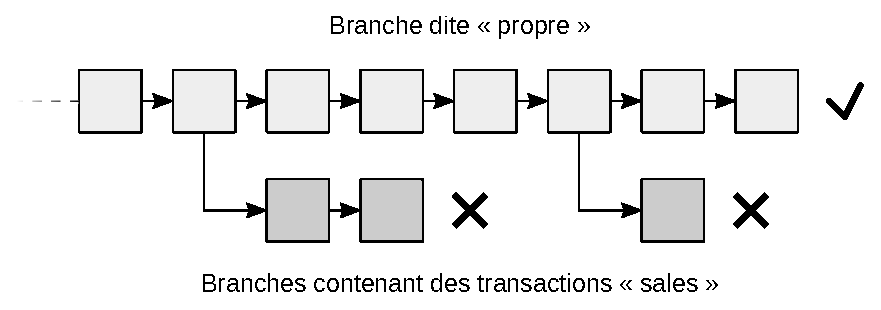
\includegraphics[scale=0.7]{img/mining-attack-censorship.eps}
  \caption{Attaque de censure active.}
  \label{fig:censorship-attack}
\end{figure}

% Cinq statégies de minage :
% - Censure : le mineur applique systématiquement la censure en rejettant les blocs contenant les transactions sales
% - Suivisme honnête : le mineur n'applique pas la censure active, applique la censure passive et prolonge la chaîne la plus longue en privilégiant le premier bloc reçu
% - Suivisme malhonnête : le mineur n'applique pas la censure active, applique la censure passive et prolonge la chaîne la plus longue en privilégiant la branche des censeurs
% - Suivisme dissident : le mineur n'applique pas la censure active, applique la censure passive et prolonge la chaîne la plus longue en privilégiant la branche des dissidents
% - Dissidence : le mineur n'applique ni la censure active, ni la censure passive, et prolonge systématiquement la branche concurrente à celle des censeurs, même si elle est plus courte

% Coût de l'attaque
Le coût d'une telle attaque peut être colossal suivant la puissance de calcul déployée sur le réseau\sendnote{On a vu dans le chapitre~\ref{ch:confirmation} que le coût d'une telle attaque se chiffre en milliards de dollars sur le réseau Bitcoin principal.}. Mais ce coût serait justifié par le développement des activités illégales évitant l'impôt et le seigneuriage. En effet, comme montré dans le chapitre~\ref{ch:adversaire}, le profil-type de l'attaquant est l'État dont le pouvoir de prélèvement repose grandement sur son contrôle de la monnaie~: c'est pourquoi il se moque de réduire (voire de détruire) l'utilité de Bitcoin ce faisant.

% Intensification du conflit (guerre contre Bitcoin, marché noir)
Cette attaque hypothétique serait précédée d'une déclaration de guerre contre Bitcoin. Toute la tolérance vis-à-vis des utilisateurs disparaîtrait, et ce qui n'était pas officiel le deviendrait~: toutes les transactions qui ne sont pas explicitement autorisées seraient déclarées interdites. L'utilisation libre serait criminalisée d'une manière ou d'une autre, et le minage honnête aussi.

% Cela s'accompagnerait probablement d'une mise en avant d'une alternative~: soit une version plus conforme de Bitcoin, soit une monnaie numérique de banque centrale (MNBC), présentée comme plus sûre et moins volatile.

% Cooptation, déploiement de matériel et attaque
Ce durcissement permettrait de coopter plus largement les regroupements miniers auxquels les directives étatiques seraient transmises. L'État pourrait aussi réquisitionner ou acheter son propre matériel de hachage. En somme, il disposerait à un moment donné d'une puissance de calcul majoritaire. Une fois la puissance de calcul rassemblée, l'attaque serait mise à exécution.

% Prolongement de l'attaque
La censure active est insidieuse car il suffit que 51~\% l'applique pour qu'elle continue. Son prolongement dans le temps peut finir par constituer une nouvelle normalité. Par conséquent, les mineurs économiquement rationnels ont tout intérêt à appliquer la censure, comme l'a montré un article de Juraj Bednar sur le sujet\sendnote{Juraj Bednar, \eng{Bitcoin censorship will most likely come, pt 2}, 18 novembre 2020~: \url{https://juraj.bednar.io/en/blog-en/2020/11/18/bitcoin-censorship-will-most-likely-come-pt-2/}.}. L'attaquant ne doit donc pas nécessairement disposer en permanence de la majorité du taux de hachage.

% Cas extrême, attaque Goldfinger
La confidentialité n'empêche pas la censure d'avoir lieu, mais la rend simplement plus coûteuse. Dans le cas où l'intégralité des utilisateurs refuserait de se conformer aux normes de surveillance, les censeurs devraient refuser l'ensemble des transactions et ne pas recevoir les frais correspondants. L'attaque prendrait alors la forme d'une destruction totale de l'utilité de la chaîne par le minage de blocs vides, c'est-à-dire une attaque Goldfinger. Le nom de cette dernière fait référence au principal antagoniste du film de James Bond éponyme sorti en 1964, qui souhaitait irradier le stock d'or américain sécurisé au dépôt de Fort Knox dans le but de le rendre durablement inutilisable et d'augmenter la valeur du reste de l'or\sendnote{Joshua A. Kroll, Ian C. Davey, Edward W. Felten, «~\eng{The Economics of Bitcoin Mining, or Bitcoin in the Presence of Adversaries}~», in \eng{Workshop on the Economics of Information Security}, 2013~: \url{https://asset-pdf.scinapse.io/prod/2188530018/2188530018.pdf}.}.

% Censure et résistance
\clearpage
De ce fait, il est tout à fait possible d'exercer de la censure dans Bitcoin. Toutefois, ce n'est ni facile, ni définitif, car il existe un mécanisme au sein du protocole permettant de lutter contre ce type d'attaque~: la résistance à la censure.

\section*{Le mécanisme de résistance à la censure}
\addcontentsline{toc}{section}{Le mécanisme de résistance à la censure}

% Définition de la résistance à la censure
La résistance à la censure désigne la difficulté à entraver arbitrairement les transactions. Elle est couramment citée comme l'une des deux grandes promesses de Bitcoin~: permettre à quiconque d'envoyer des fonds à n'importe qui d'autre, quel que soit le moment, où que se trouve le destinataire dans le monde, pourvu qu'il dispose d'un accès à Internet.

% La résistance à la censure est essentielle
La résistance à la censure constitue un élément essentiel de Bitcoin. Si elle n'existait pas, le système ne pourrait tout simplement pas survivre en tant que tel~: il deviendrait un système contrôlé centralement par une autorité décidant des bonnes et des mauvaises transactions. Il devrait s'adapter, tel GoldMoney ou PayPal, ou périr, à l'instar de e-gold ou de Liberty Reserve. De plus, le pouvoir absolu sur la sélection des transactions permettrait à cette autorité d'exercer \eng{de facto} une influence irrésistible sur le protocole par le biais de l'application de soft forks (comme nous le verrons dans les chapitres \ref{ch:changement} et \ref{ch:determination}), ce qui mènerait \emph{in fine} à la destruction de la politique monétaire originelle. Sans résistance à la censure, la proposition de valeur de Bitcoin s'effondrerait.

% Pas de description par Satoshi
Cependant, cette résistance n'a jamais été décrite explicitement par Satoshi Nakamoto. Dans ses interventions, le père de Bitcoin a expliqué comment son système était sécurisé économiquement contre la double dépense, ce qui était déjà une grande évolution par rapport aux modèles décentralisés précédents. Mais il n'a en revanche pas indiqué comment le système pouvait s'opposer à la censure, c'est-à-dire au blocage partiel ou total de l'activité transactionnelle par une entité hostile. Il semblait se reposer sur la bonne volonté des mineurs «~honnêtes~», pensant même qu'il y aurait «~probablement toujours des nœuds prêts à traiter les transactions gratuitement\sendnote{Satoshi Nakamoto, \eng{Bitcoin v0.1 released}, \wtime{08/01/2009 19:27:40 UTC}~: \url{https://www.metzdowd.com/pipermail/cryptography/2009-January/014994.html}.}~», cette résistance allant de soi.

% Mécanisme de résistance à la censure mis en lumière par Eric Voskuil
Le mécanisme de résistance à la censure de Bitcoin a été mis en lumière en 2018, par le développeur et auteur Eric Voskuil, qui a montré qu'il reposait de manière essentielle sur les frais de transaction\sendnote{Le mécanisme de résistance à la censure a initialement été décrit par Eric Voskuil en janvier 2018~: \url{https://github.com/libbitcoin/libbitcoin-system/wiki/Other-Means-Principle/77d7556a14f89d1704f1bb97ca0aed04606363d0}. Voir aussi Eric Voskuil, «~Propriété de résistance à la censure~», in \emph{Cryptoéconomie~: Principes fondamentaux de Bitcoin}, Amazon KDP, 2022, pp. 24--25.}. Comme dans le cas de la résistance à la double dépense, la propriété de résistance à la censure n'est pas absolue mais économique~: c'est une régulation financée par les frais des transactions prohibées.

% Principe de la majorité
\clearpage
La sécurité minière, on le rappelle, repose sur un principe majoritaire~: la quantité de puissance de calcul contrôlée par les mineurs honnêtes doit être supérieure par rapport à celle des attaquants. L'important n'est pas que le taux de hachage de Bitcoin soit le plus haut possible~; c'est que les mineurs disposant d'une puissance de calcul non négligeable soient prêts à miner systématiquement toutes les transactions payant un montant correct de frais et à toujours construire leurs blocs à partir de la plus longue chaîne. % Pas de censue passive et pas de recoordination de chaîne

% Sécurité = activité × distribution × participation
Ainsi, cette sécurité ne dépend pas uniquement de la puissance de calcul. Elle est aussi fonction de la distribution de cette puissance de calcul et de la fraction de mineurs par rapport au reste de l'humanité\sendnote{Eric Voskuil, «~Modèle de sécurité qualitatif~», in \emph{Cryptoéconomie~: Principes fondamentaux de Bitcoin}, Amazon KDP, 2022, pp. 59--62.}. En effet, un taux de hachage qui serait concentré dans les mains d'un seul mineur créerait une sécurité équivalente à celle d'un système centralisé, dépendante du mineur en question. Aussi, un réseau équitablement distribué et déployant une grande quantité puissance de calcul aura plus de risque d'être coopté s'il comporte un petit nombre de mineurs que s'il en comporte un grand nombre.

% Compensation du risque
La solution au problème de la censure provient des mineurs dissidents, qui sont prêts à confirmer des transactions litigieuses ou décrétées comme illégales par le pouvoir. Le risque pris par ces mineurs doit alors être compensé économiquement.

% Anonymat du mineur
Le mineur dissident a besoin de rester anonyme afin de pouvoir miner dans la clandestinité. Cette possibilité est assurée par le fait que les mineurs ne sont jamais contraints de s'identifier au sein du protocole. Le signalement des blocs minés par les coopératives minières est en effet une démarche purement optionnelle et volontaire, ayant pour but de rassurer les utilisateurs (leurs clients) sur la distribution du système.

% Rôle de la création monétaire
La part du revenu du minage provenant de la création monétaire joue un rôle accessoire dans la lutte contre la censure, que cette dernière soit passive ou active. D'une part, cette partie de la récompense est la même pour tous les mineurs, ce qui fait qu'elle n'influe pas sur leur choix économique d'inclure une transaction ou non dans un bloc. D'autre part, la potentielle chute de l'utilité (et donc du revenu de minage) du système provoquée par une censure active (attaque), ne saurait empêcher l'autorité à l'origine d'arriver à ses fins. Les motivations de cette dernière sont en effet particulières~: elle ne cherche pas à réaliser un profit direct mais à contrôler, voire détruire, le système en décrétant quelles transactions sont autorisées et lesquelles ne le sont pas.

% Rôle des frais
En revanche, les frais de transaction sont, eux, essentiels au mécanisme de résistance à la censure. Par leur intégration dans le protocole, ces commissions sont chacunes associées publiquement à une transaction. Ainsi, les frais luttent d'une part contre la censure passive en incitant les mineurs à confirmer les transactions, et découragent d'autre part la censure active en donnant à la branche censurée une importance économique plus grande.

% Intégration des frais
% Les frais sont intégrés au protocole. Ils sont donc généralement l'association directe avec la transaction. Ceux-ci peuvent être payés directement par les clients qui envoient les transactions, ou ils peuvent être indirectement pris en charge par les commerçants au moyen de l'application d'une réduction sur le prix des biens vendus.

% Attaque
Dans le cas d'une attaque de censure active, les censeurs acquièrent plus de la moitié de la puissance de calcul du réseau et rejettent ouvertement un groupe de transactions défini (par une liste noire par exemple) en refusant les blocs qui contiendrait l'une d'entre elles. La chaîne des censeurs est considérée par les nœuds honnêtes comme la chaîne correcte car elle est plus longue.

% Réaction
C'est dans ce contexte que le mécanisme des frais intervient. Les initiateurs des transactions censurées, voyant que leurs transactions ne sont pas confirmées, augmentent leurs commissions. C'est un comportement naturel que l'on observe déjà lors des périodes de congestion du réseau, comme au sommet de la bulle de 2017, lorsque les frais médians par transaction ont dépassé les 30~\$\pagenote{«~lorsque les frais médians par transaction ont dépassé les 30~\$~»~: \url{https://bitinfocharts.com/comparison/bitcoin-median_transaction_fee.html\#alltime}.}. En outre, il est logique de payer une grande quantité de frais pour transférer de fortes sommes, celles-ci étant plus à risque que les petits transferts\sendnote{Dans Bitcoin, les frais sont aujourd'hui payés proportionnellement à la charge des données (taille ou poids de la transaction). Cependant, la menace de plus en plus claire de la censure pourrait pousser les utilisateurs à payer des frais proportionnels au montant transféré comme cela se fait dans le domaine financier en général.}.

% Supplément de frais
Cette augmentation crée un supplément de frais, qui constitue la différence entre les frais de toutes les transactions et ceux des transactions non autorisées qui se retrouvent dans les mempools des nœuds honnêtes. C'est ce supplément (et ce supplément uniquement) qui incite les mineurs dissidents à déployer plus de puissance de calcul au cours du temps~: plus l'économie supprimée est importante, plus le différentiel de puissance de calcul résultant est grand.

% Riposte
Les mineurs dissidents se coordonnent en privé ou par la voie d'un signalement pour planifier une riposte. Une fois que la puissance de calcul est jugée suffisante, ils se mettent à confirmer les transactions censurées. Puisque leur puissance de calcul est majoritaire, leur chaîne devient la plus longue et la chaîne des censeurs est invalidée. De cette manière, la censure est vaincue, du moins jusqu'à une nouvelle offensive de l'ennemi.

% Mécanisme ancré dans le protocole
Ainsi, le mécanisme de résistance à la censure est ancré profondément dans le protocole. La preuve de travail, le caractère anonyme du minage, le système de frais intégré~: ce sont autant d'éléments permettant de coordonner un marché des frais afin de repousser les censeurs. Il est impossible d'estimer quelle serait la part de l'économie censurée, l'envergure de l'attaque étatique ou le montant de frais que les utilisateurs seraient prêts à payer, de sorte qu'on ne peut pas garantir l'incensurabilité de Bitcoin. Mais le mécanisme n'en est pas moins fonctionnel.

% Négligence du rôle des frais de transactions
Il est à noter que le rôle des frais de transaction, explicité en 2018 par Eric Voskuil, a été négligé par certains protocoles cryptoéconomiques. C'est en particulier le cas d'Ethereum qui a fait le choix de brûler une partie des frais du réseau dans le but de rendre l'éther déflationniste au sens monétaire avec l'activation de l'EIP-1559 en août 2021\pagenote{«~l'activation de l'EIP-1559 en août 2021~»~: Ludovic Lars, \emph{Ethereum face à une catastrophe annoncée~? Censure et volatilité~: l'EIP-1559, le cauchemar des mineurs}, 15 juillet 2021~: \url{https://journalducoin.com/analyses/eip-1559-changement-nefaste-ethereum/}.}. La communauté d'Ethereum a également choisi de passer en preuve d'enjeu en septembre 2022, ce qui constitue un autre pas vers l'acceptation de la censure comme nous l'expliquerons plus bas.

\vspace{-1em}
\section*{L'importance de la confidentialité}
\addcontentsline{toc}{section}{L'importance de la confidentialité}

La censure financière est étroitement apparentée à la surveillance des transactions. Cette dernière permet en effet d'affiner la sélection des transferts et d'exercer un pouvoir subtil sur l'économie, sans brusquer les personnes les plus dociles. La chose vaut pour le monde bancaire comme nous l'avons constaté, mais elle vaut aussi pour Bitcoin.

% --- Deux manières de protéger sa richesse ---

% Défense physique
Il existe deux manières de protéger sa richesse et sa liberté~: par la force physique et par la dissimulation. La première méthode consiste à se prémunir contre le vol directement en défendant soi-même ses biens (si besoin à l'aide d'une arme à feu), ou bien indirectement par le recours aux services de police étatiques ou aux services de protection privés (gardes du corps, quartiers sécurisés, agence de protection), très prisés des personnes très fortunées. Cette méthode est importante et utile contre les criminels communs, mais elle est relativement inefficace contre la puissance dominante locale dont nous sommes à la merci -- l'État.

% Défense par dissimulation
C'est pourquoi les individus ont plus souvent recours à la seconde méthode, qui consiste à dissimuler leur richesse pour ne pas qu'autrui en ait connaissance et puisse s'en emparer directement. Cela permet de dissuader le voleur usant la menace de violence d'aller plus loin~: il pourrait nous interroger pour savoir où se trouve notre richesse, mais cette action représenterait un coût supplémentaire (proportionnel à notre refus de lui livrer cette information) qui freinerait sa recherche.

% Définition de la confidentialité
Cette méthode est directement liée à la confidentialité (aussi appelée \eng{privacy} ou protection de la vie privée) qui est le fait de réserver des informations à un petit nombre de personnes déterminées. La confidentialité est distincte du secret dans le sens où la personne peut choisir de révéler sélectivement des informations (confidence). Dans le contexte financier, il s'agit généralement de faire en sorte que les détails d'une transaction ne soient connus que des participants.

% La confidentialité crée la liberté individuelle
La confidentialité forme la base de la liberté individuelle dans la société et constitue une caractéristique essentielle pour tout le monde. Elle sert en effet à \emph{créer une asymétrie} entre le faible et le fort, entre l'individu et l'État, de sorte que ce dernier ne puisse pas empiéter absolument sur les droits du premier. L'État veut vous persuader du contraire, en vous disant que vous n'avez rien à craindre si vous n'avez rien à cacher\sendnote{«~Je dis que quiconque tremble en ce moment est coupable~; car jamais l'innocence ne redoute la surveillance publique.~» -- Maximilien de Robespierre, \emph{Discours du 11 germinal, an II}, 31 mars 1794.}, mais il n'y a rien d'historiquement plus faux, comme l'ont montré les exemples des totalitarisme du \textsc{xx}\ieme{}~siècle.

% --- Lien entre résistance à la censure et confidentialité ---

De ce fait, puisque la censure financière est issue de l'initiative étatique, la résistance à la censure est en général intrinsèquement liée à la confidentialité.

% Confidentialité => résistance à la censure
D'une part, la résistance à la censure de l'utilisateur individuel repose sur la confidentialité du système. Si l'État connaît toutes les transactions, il peut sanctionner l'utilisateur pour avoir effectué une transaction non autorisée, quand bien même celle-ci serait confirmée par le réseau. Certains promoteurs de BTC mettent en avant la transparence du protocole, en la présentant comme un avantage par rapport aux systèmes bancaires opaques, en insistant sur le pseudonymat et en réservant la propriété d'anonymat aux «~cryptomonnaies confidentielles~» comme Monero. Mais il s'agit d'une mécompréhension du rôle de cette transparence~: les données dans Bitcoin sont publiques dans le but unique d'assurer le consensus et l'audit, et Monero ne fait qu'implémenter un compromis différent sur le degré de transparence des transactions.

% Résistance à la censure => confidentialité
D'autre part, la confidentialité de l'utilisateur dépend de la résistance à la censure du système. En effet, si l'État dispose d'un contrôle total sur la sélection des transactions, alors il peut choisir de ne confirmer que les transactions qui dévoilent l'identité de l'expéditeur et celle du destinataire. Cette dépendance est souvent remise en question par certains partisans de Monero qui estiment que la confidentialité par défaut du système protège les utilisateurs de la censure, considérant que l'État ne peut pas censurer une transaction qu'il ne connaît pas. Néanmoins, cette vision est plutôt naïve car les utilisateurs ont la possibilité technique de révéler les informations relatives à leurs adresses aux organismes de surveillance\sendnote{Dans Monero et dans les systèmes apparentés, la révélation des transactions liées à une adresse se fait par l'intermédiaire d'une clé privée d'inspection (\eng{private view key}).}~; la seule barrière à cela est le coût supplémentaire qu'une telle surveillance représente. % C'est pour cette raison qu'un État pourrait choisir de refuser toute transaction non transparente. La résistance à la censure dépend aussi du coût de l'attaque, qui serait beaucoup moins coûteuse à réaliser dans le cas de Monero, probablement 200 fois moins que sur BTC (mars 2023).

% Interdépendance de la confidentialité et de la résistance à la censure
La confidentialité et la résistance à la censure sont donc interdépendantes dans Bitcoin. Sans confidentialité, il n'y a pas de résistance à la censure individuelle~; et sans résistance à la censure, il n'y a pas de confidentialité individuelle. C'est pour cette raison que la surveillance généralisée, loin d'être anodine, constitue un problème majeur.

% État des lieux de la surveillance des intermédiaires
La surveillance s'est étendue dans Bitcoin au cours de son développement économique par la réglementation des intermédiaires financiers. Les plateformes de change entre monnaies traditionnelles et cryptomonnaies ont été progressivement contraintes d'appliquer des normes de connaissance du client (KYC) et de lutte contre le blanchiment (AML) similaires au système bancaire classique. Cette récupération d'informations s'est accompagnée de l'émergence de sociétés d'analyses de chaîne, telles que Chainalysis ou Ciphertrace, qui croisent les données d'identification avec les évènements de la chaîne de blocs de façon à en dégager une interprétation probable, et qui fournissent les résultats à leurs clients qui sont les agences étatiques, les institutions financières et les grandes entreprises du domaine. En outre, l'étau est encore en train de se resserrer, avec l'apparition d'une version modifiée de la «~règle du voyage~» (\eng{Travel Rule}), recommandée par le GAFI et déjà imposée par la FINMA suisse, qui consiste pour un intermédiaire à vérifier systématiquement l'adresse de retrait du client\sendnote{Dans le monde bancaire, la \eng{Travel Rule} a originellement été promulguée par le FinCEN étasunien en 1996 (voir 31 CFR 103.33(g)). Elle exige que toutes les institutions financières transmettent des informations sur les expéditeurs à l'institution financière suivante lors de certains transferts de fonds. Dans le cas de Bitcoin et des cryptomonnaies, il s'agit d'émuler ce voyage en considérant que les utilisateurs sont des institutions financières lorsqu'ils réalisent des transactions souveraines. Le GAFI a ajouté le transfert d'«~actifs virtuels~» à ses recommandations en juin 2019, notamment en ce qui concerne la recommandation 16. Cette règle du voyage cryptomonétaire pourrait être appliquée par l'intégration dans les portefeuilles du protocole de preuve de propriété d'adresse (AOPP) proposé en janvier 2022.}\pagenote{«~l'apparition d'une version modifiée de la "règle du voyage", recommandée par le GAFI et déjà imposée par la FINMA suisse~»~: \url{https://www.fincen.gov/sites/default/files/advisory/advissu7.pdf} -- Recommandation 16 du GAFI, mise à jour en juin 2019 pour inclure le transferts d'actifs virtuels~: \url{https://www.fatf-gafi.org/fr/publications/Recommandationsgafi/Recommandations-gafi.html}. -- \url{https://www.finma.ch/en/news/2019/08/20190826-mm-kryptogwg/} -- \url{https://aopp.group/}.}.

% Lutte contre la surveillance
Cette évolution crée une réelle menace sur Bitcoin en général. C'est pourquoi il se forme en face une résistance visant à déjouer la surveillance, notamment par l'intermédiaire de techniques d'amélioration de la confidentialité. C'est le cas par exemple du mélange de pièces, ou CoinJoin, qui permet de brouiller les pistes. C'est aussi le cas des méthodes intégrées dans Monero. Nous développerons cet aspect dans le chapitre~\ref{ch:rouages}. % Mais ces méthodes doivent être utilisées, et elles doivent rester à jour de l'avancée de la surveillance.

% Importance de la confidentialité
Ainsi, la confidentialité est essentielle pour préserver sa richesse et son autonomie. On ne peut pas être réellement libre sans protéger sa vie privée. Comme l'écrivait le fabuliste Florian~: «~Pour vivre heureux vivons cachés\sendnote{Jean-Pierre Claris de Florian, «~Le Grillon~», in \emph{Fables de Florian}, 1793.}.~»

\section*{Les interventions humaines dans le consensus}
\addcontentsline{toc}{section}{Les interventions humaines dans le consensus}

La possibilité de censure dans Bitcoin provoque généralement une volonté de trouver une solution, s'inscrivant dans la démarche d'ingénieur qui caractérise les amateurs de cryptomonnaie. Beaucoup de personnes sont en effet séduites par une alternative à la régulation par les frais~: l'intervention humaine directe sur la chaîne. Celle-ci consiste à recourir au «~consensus social\pagenote{«~consensus social~»~: Arthur Breitman parlait de \eng{social consensus} dès août 2014 dans la première description formelle de Tezos. -- Arthur Breitman, \eng{Tezos: A Self-Amending Crypto-Ledger}, 3 août 2014~: \url{https://tezos.com/position-paper.pdf}.}~», c'est-à-dire au mécanisme de détermination du protocole. Deux idées de ce type semblent avoir un certain succès~: l'UASF anti-censure et l'UAHF de changement de preuve de travail. Il s'agit cependant d'une tentation dangereuse comme nous allons essayer de le montrer.

% Lorsqu'on parle de la possibilité de censure, une autre alternative a tendance à séduire les personnes qui n'ont pas suffisamment creusé la question~: celle d'intervenir socialement sur la chaîne. Il s'agit d'avoir recours au «~consensus social\sendnote{Pour reprendre l'expression d'Arthur Breitman utilisée dans la première description formelle de Tezos en août 2014. -- Arthur Breitman, \eng{Tezos: A Self-Amending Crypto-Ledger}, 3 août 2014~: \url{https://tezos.com/position-paper.pdf}.}~», c'est-à-dire le mécanisme de détermination du protocole.

% --- UASF anti-censure ---

La première idée est de rejeter la censure en invalidant la branche des censeurs partiellement ou totalement, c'est-à-dire en portant atteinte au principe de la chaîne la plus longue. Le rejet peut se faire en rendant les blocs de la chaîne des censeurs invalides ou en imposant la validité de la chaîne concurrente par un point de contrôle temporaire. Une telle mesure constitue un soft fork (à savoir une restriction des règles de consensus) et doit être activée par les utilisateurs à un horodatage ou à une hauteur de bloc donné, d'où le fait qu'on la désigne comme un \eng{User Activated Soft Fork} (UASF). Elle provoque une scission car elle n'est pas, dans le cas précis de la censure, soutenue par la majorité de la puissance de calcul.

% Vitalik
L'idée d'invalider la censure par consensus social était déjà évoquée par Vitalik Buterin en 2016 dans le cas de la preuve d'enjeu~:

\begin{quote}
«~Sur des échelles de temps moyennes à longues, les humains sont assez bons pour le consensus. Même si un adversaire avait accès à une puissance de hachage illimitée, et qu'il parvenait à réaliser une attaque des 51~\% contre une chaîne de blocs majeure en inversant ne serait-ce que le dernier mois d'histoire, il serait beaucoup plus difficile de convaincre la communauté que cette chaîne est légitime que de simplement distancer la puissance de hachage de la chaîne principale. [...] Ces considérations sociales sont ce qui protège finalement toute chaîne de blocs à long terme, que la communauté de cette chaîne de blocs l'admette ou non (notez que Bitcoin Core admet cette primauté de la couche sociale)\sendnote{Vitalik Buterin, \eng{A Proof of Stake Design Philosophy}, 30 décembre 2016~: \url{https://medium.com/@VitalikButerin/a-proof-of-stake-design-philosophy-506585978d51}.}.~»
\end{quote}

% "On medium to long time scales, humans are quite good at consensus. Even if an adversary had access to unlimited hashing power, and came out with a 51\% attack of any major blockchain that reverted even the last month of history, convincing the community that this chain is legitimate is much harder than just outrunning the main chain's hashpower. They would need to subvert block explorers, every trusted member in the community, the New York Times, archive.org, and many other sources on the internet; all in all, convincing the world that the new attack chain is the one that came first in the information technology-dense 21st century is about as hard as convincing the world that the US moon landings never happened. These social considerations are what ultimately protect any blockchain in the long term, regardless of whether or not the blockchain's community admits it (note that Bitcoin Core does admit this primacy of the social layer).
%
% However, a blockchain protected by social consensus alone would be far too inefficient and slow, and too easy for disagreements to continue without end (though despite all difficulties, it has happened); hence, economic consensus serves an extremely important role in protecting liveness and safety properties in the short term."

% Invalidation des blocs des censeurs
Cette mesure peut être mise en place par une invalidation directe mais celle-ci n'est facile à implémenter que si les censeurs marquent leurs blocs d'une manière ou d'une autre\pagenote{«~invalidation directe~»~: Cette méthode peut par exemple être mise en place dans l'esprit de l'\eng{User Resisted Soft Fork} proposé par Michael Folkson en avril 2022 en réaction à la menace d'activation de la mise à niveau \longstring{OP\_CHECKTEMPLATEVERIFY}. -- Michael Folkson, \eng{[bitcoin-dev] User Resisted Soft Fork for CTV}, \wtime{21/04/2022 16:45:20 UTC}~: \url{https://lists.linuxfoundation.org/pipermail/bitcoin-dev/2022-April/020262.html}.}. Cela a été réalisé par Bitcoin ABC le 1\ier{} décembre 2020 sur sa chaîne nouvellement créée pour contrer la censure active d'un mineur mécontent de la scission avec Bitcoin Cash\sendnote{Un seul bloc (le bloc 662~687 d'identifiant \longstring{00000000000000000709b858a6a0c8610e604e77072ef4407763afb0780ce712}) de l'attaquant a été invalidé, faisant que 172 blocs ont été mis de côté, et que la chaîne non censurée est devenue la chaîne correcte. -- Nikita Zhavoronkov sur Twitter, \wtime{01/12/2020 21:59 UTC}~: \url{https://twitter.com/nikzh/status/1333893457920876550}.}.

% Point de contrôle
Il est aussi possible d'inclure un point de contrôle (\eng{checkpoint}) dans le protocole. Un point de contrôle est un bloc considéré comme valide par défaut. Ce mécanisme a été implémenté dans le logiciel de Bitcoin dès juillet 2010 dans le but d'éviter une recoordination de chaîne\pagenote{«~implémenté dans le logiciel de Bitcoin dès juillet 2010~»~: Satoshi Nakamoto, \eng{Bitcoin 0.3.2 released}, \wtime{17/07/2010 21:35:51 UTC}~: \url{https://bitcointalk.org/index.php?topic=437.msg3807\#msg3807}.} et certains de ces points de contrôle sont encore présents dans Bitcoin Core\sendnote{Le point de contrôle le plus récent est celui du bloc 295~000 miné le 9 avril 2014 (au même moment de l'arrivée de Wladimir van der Laan au poste de mainteneur principal) et ayant pour identifiant \longstring{00000000000000004d9b4ef50f0f9d686fd69db2e03af35a100370c64632a983}. Voir le fichier \longstring{chainparams.cpp} dans Bitcoin Core.}\pagenote{«~certains de ces points de contrôle sont encore présents dans Bitcoin Core~»~: \url{https://github.com/bitcoin/bitcoin/blob/24.x/src/chainparams.cpp\#L148-L164}.}. Dans cette logique, il suffit d'imposer un bloc comme obligatoire pour invalider la chaîne des censeurs. Cela a été réalisé par Bitcoin SV en août 2021, qui subissait alors une censure active\sendnote{BSV Association sur Twitter, \wtime{03/09/2021 21:17 UTC}~: \url{https://twitter.com/BitcoinAssn/status/1422668065024663554}.}.

% Efficacité de l'intervention humaine
Toutefois, même si ce type de recours peut effectivement fonctionner de manière ponctuelle et temporaire, il ne constitue en rien un mécanisme robuste de résistance à la censure. En effet, il crée beaucoup trop d'instabilité en faisant en dernier lieu reposer le consensus sur l'accord social. Il offre ainsi la possibilité pour une puissance hostile de déstabiliser durablement le système en semant la zizanie dans la communauté (notamment par la pression exercée sur les relais d'opinion) et en créant par là des scissions multiples impossibles à départager par un facteur objectif.

% Pourquoi l'UASF anti-censure est une mauvaise idée
\clearpage
L'intervention directe de l'accord social dans la confirmation des transactions est par conséquent une très mauvaise idée. Même dans les cas où les participants sont d'accord pour dire qu'un tel évènement est indésirable, ils sont souvent en total désaccord sur la manière de traiter le problème, ainsi qu'on l'a observé lors de la scission entre Ethereum et Ethereum Classic. Les être humains sont capables de se mettre d'accord à long terme, comme le témoigne la convergence vers un petit nombre de langues, de religions, de monnaies, etc. Néanmoins, à court terme ce n'est très certainement pas le cas. D'où le recours au mécanisme de consensus automatisé qu'est le minage.

% --- UAHF de changement de preuve de travail de preuve de travail ---

Une autre mesure proposée, moins subjective mais plus perturbatrice, est la modification de la fonction de preuve de travail. Celle-ci permet de faire cesser l'attaque à court terme puisqu'elle rend le matériel spécialisé des censeurs obsolète, leur faisant supporter une lourde perte au passage. Il s'agit d'un hard fork (à savoir une modification incompatible des règles de consensus) qui doit être activé par les utilisateurs à un horodatage ou à une hauteur de bloc donné, c'est-à-dire un \eng{User Activated Hard Fork} (UAHF). Cette option extrême a été soutenue par les développeurs luke-jr et Gregory Maxwell lors de la guerre des blocs en 2015 -- 2016\pagenote{«~soutenue par les développeurs luke-jr et Gregory Maxwell~»~: \url{https://www.reddit.com/r/Bitcoin/comments/3fg0jw/could_a_cartel_of_pool_operators_collude_to/ctoat0d/}~;\url{https://www.reddit.com/r/bitcoinxt/comments/41pbmf/maxwell_considers_changing_the_pow_algorithm_in/}.}. Elle a également été défendue par le développeur en chef de Bitcoin ABC Amaury Séchet en novembre 2018 qui l'a qualifiée d'«~option nucléaire [...] de dernier recours\sendnote{Amaury Séchet (deadalnix) sur Twitter, \wtime{12/11/2018 11:42 UTC}~: \url{https://twitter.com/deadalnix/status/1061947426096009216}.}~».

% Pourquoi le hard fork de changement de preuve de travail est une mauvaise idée
De même que dans le cas de l'invalidation de la censure par intervention sociale, il s'agit d'une mesure plus néfaste à long terme que le statu quo. Premièrement, la perte subie par les censeurs est aussi encaissée par les mineurs honnêtes et dissidents. Deuxièmement, l'économie est répartie entre deux chaînes distinctes, réduisant l'utilité monétaire totale. Troisièmement, le coût d'une attaque est drastiquement réduit à court terme. Quatrièmement, les mineurs perdent confiance dans le protocole et doivent s'assurer contre le risque d'un nouveau changement, réhaussant le coût de la sécurité minière par rapport au coût de l'attaque. Et cinquièmement, la nouvelle distribution du minage n'est pas forcément meilleure que l'ancienne, les gros mineurs pouvant déployer du capital plus facilement.

% Effet néfaste de l'intervention humaine
De manière générale, l'intervention humaine à court terme est loin d'être désirable. Si la chaîne subit une attaque minière, il est probable qu'elle soit aussi attaquée au niveau social. Les interventions ont ainsi toutes les chances de se multiplier, faisant sombrer la chaîne dans une spirale de scissions et la menant à l'insignifiance économique. Le cas de Bitcoin Cash est le plus éclairant~: en raison de hard forks programmés tous les six mois, la chaîne a subi deux scissions majeures après sa séparation avec Bitcoin-BTC (en 2018 avec BSV et en 2020 avec XEC), ce qui a mené l'ensemble à être valorisé à moins de 1~\% de la valeur agrégée du BTC. En outre, si ce caractère néfaste est valable pour les cryptomonnaies en construction, qui peuvent se permettre ces interventions en raison de la petitesse et de l'homogénéité de leur économie, elle l'est d'autant plus pour une version mature de Bitcoin qui soutiendrait une économie plus grande et plus diversifiée.

\section*{Les variantes des consensus par preuve de travail}
\addcontentsline{toc}{section}{Les variantes des consensus par preuve de travail}

% Alternatives, variantes
Le risque de censure a également inspiré le développement d'algorithmes de consensus alternatifs à celui de Bitcoin. L'alternative la plus connue est la preuve d'enjeu, qui sera décrite dans la section suivante. Les autres alternatives sont des variantes de l'algorithme de Nakamoto par preuve de travail, dont les trois principales sont le minage combiné, la preuve d'espace et la finalisation anticipée. % protection contre la recoordination profonde, "checkpoints automatiques"

% --- Minage combiné ---

La première proposition est le minage combiné\pagenote{«~le minage combiné~»~: Aljosha Judmayer, Alexei Zamyatin, Nicholas Stifter, Artemios G.  Voyiatzis, Edgar Weippl, \eng{Merged Mining: Curse of Cure?}, 22 août 2017~: \url{https://eprint.iacr.org/2017/791}.}. Le minage combiné, ou \eng{merge mining} en anglais, est l'action de miner plusieurs chaînes en simultané par la réutilisation du travail fourni sur une chaîne parente pour la validation des chaînes filles ou auxiliaires.

Le procédé a été décrit par Satoshi Nakamoto en décembre 2010, dans un message concernant BitDNS, le projet de système distribué de noms de domaine à l'origine de Namecoin. Le créateur de Bitcoin écrivait ainsi sur le forum~:

\begin{quote}
«~Je pense qu'il serait possible que BitDNS forme un réseau complètement séparé et possède une chaîne de blocs distincte, tout en partageant la puissance de calcul avec Bitcoin. Le seul chevauchement consisterait à faire en sorte que les mineurs puissent rechercher des preuves de travail pour les deux réseaux simultanément.

Les réseaux n'auraient besoin d'aucune coordination. Les mineurs adhéreraient aux deux réseaux en parallèle. Ils scanneraient SHA de telle sorte que s'ils obtenaient un résultat, ils pourraient résoudre les deux en même temps. Une solution pourrait concerner un seul des réseaux si l'un d'eux présente une difficulté moindre.

Je pense qu'un mineur externe pourrait appeler getwork sur les deux programmes et combiner le travail. Peut-être appeler Bitcoin, en tirer du travail, le remettre à getwork sur BitDNS pour le combiner en un travail commun.

Au lieu d'une fragmentation, les réseaux partageraient et augmenteraient la puissance de calcul totale de chacun. Cela résoudrait le problème des réseaux multiples, qui constituent un danger les uns pour les autres si la puissance de calcul disponible se concentre sur l'un d'entre eux. Au lieu de cela, tous les réseaux du monde partageraient la puissance de calcul combinée, augmentant ainsi la puissance totale. Il serait plus facile pour les petits réseaux de se lancer en puisant dans une base existante de mineurs\sendnote{Satoshi Nakamoto, \eng{Re: BitDNS and Generalizing Bitcoin}, \wtime{09/12/2010 21:02:42 UTC}~: \url{https://bitcointalk.org/index.php?topic=1790.msg28696\#msg28696}.}.~»
\end{quote}

% "I think it would be possible for BitDNS to be a completely separate network and separate block chain, yet share CPU power with Bitcoin.  The only overlap is to make it so miners can search for proof-of-work for both networks simultaneously.
%
% The networks wouldn't need any coordination.  Miners would subscribe to both networks in parallel.  They would scan SHA such that if they get a hit, they potentially solve both at once.  A solution may be for just one of the networks if one network has a lower difficulty.
%
% I think an external miner could call getwork on both programs and combine the work.  Maybe call Bitcoin, get work from it, hand it to BitDNS getwork to combine into a combined work.
%
% Instead of fragmentation, networks share and augment each other's total CPU power.  This would solve the problem that if there are multiple networks, they are a danger to each other if the available CPU power gangs up on one.  Instead, all networks in the world would share combined CPU power, increasing the total strength.  It would make it easier for small networks to get started by tapping into a ready base of miners."

% Preuves de travail auxiliaires
Le minage combiné consiste à réutiliser des preuves de travail partielles d'une chaîne mère comme des preuves de travail valides sur une chaîne fille. Ces preuves de travail, dite «~auxiliaires~» et abrégées en AuxPOW, sont des sous-produits du minage de la chaîne mère, et ne nécessitent pas de dépense d'énergie supplémentaire. La seule charge imposée par le minage combiné est la gestion de la chaîne fille.

% Récompense des mineurs de la chaîne fille
Les mineurs de la chaîne fille reçoivent des récompenses supplémentaires qui sont constituées de la création monétaire locale (si la chaîne utilise une nouvelle unité de compte) et des frais de transaction. Les mineurs de la chaîne mère sont donc incités à tirer profit de cette nouvelle manne. La chaîne fille peut de ce fait disposer d'un taux de hachage conséquent assez rapidement.

% Applications : facilitation de l'amorçage, chaîne latérale
Le minage combiné a été mis en avant comme une méthode permettant de faciliter l'amorçage d'une nouvelle cryptomonnaie, en bénéficiant de l'industrie minière établie. Ce type d'algorithme de consensus a ainsi été mis en place sur Namecoin par rapport à Bitcoin et sur Dogecoin par rapport à Litecoin. Il a aussi été suggéré comme mécanisme de synchronisation des chaînes latérales. Il est ainsi implémenté de manière hybride dans RSK. Il est plus largement envisagé par Paul Sztorc dans sa proposition de Drivechain (voir chapitre~\ref{ch:scalabilite}).

% Sécurité incertaine
Cependant, l'apport en sécurité du minage combiné par rapport au minage classique est relativement faible. Le procédé permet d'augmenter le nombre d'acteurs impliqués et de restreindre les attaquants possibles (ceux-ci devant être des mineurs de la chaîne principale), mais il ne modifie pas le coût de l'attaque, qui dépend du revenu minier de cette chaîne et, dans le cas de la censure, des frais de transaction.

% Exemple du Coiledcoin
Une illustration éclatante de ce fait est l'exemple de Coiledcoin (CLC), une cryptomonnaie alternative créée en janvier 2012 qui a subi une attaque de censure fatale peu de temps après son lancement. L'attaque a été réalisée par le développeur de Bitcoin luke-jr par le biais de sa coopérative de minage, Eligius, sans qu'il n'en informe les hacheurs. Dans son message d'explication, il précisait qu'aucun membre de la coopérative n'avait subi de perte, le coût étant surtout le temps qu'il avait passé à configurer le logiciel\sendnote{luke-jr, \eng{Re: [DEAD] Coiledcoin - yet another cryptocurrency, but with OP\_EVAL!}, \wtime{06/01/2012 18:56:03 UTC}~: \url{https://bitcointalk.org/index.php?topic=56675.msg678006\#msg678006}.}.

% Effets sur la sécurité de la chaîne mère
Le minage combiné a deux effets sur la sécurité minière de la chaîne mère. D'une part, il augmente artificiellement la puissance de calcul déployée pour miner des blocs, ce qui paraît bénéfique de prime abord. Cependant, cette hausse artificielle n'agit en rien contre la censure des transactions. D'autre part, le minage combiné entraîne une centralisation de l'activité minière, en raison de la charge que représente la gestion des chaînes auxiliaires~: si les chaînes auxiliaires deviennent importantes économiquement, les mineurs de la chaîne mère n'ont d'autre choix que de les miner pour rester rentables.

% Autre variante~: «~preuve de preuve~», notamment mise en place de manière hybride par le projet Veriblock de Jeff Garzik, qui consiste à placer une représentation de l'état de la chaîne sur une chaîne de blocs parente telle que celle de BTC. Komodo's Delayed Proof Of Work.

% --- Preuve d'espace ---

La deuxième alternative est la preuve d'espace\pagenote{«~la preuve d'espace~»~: Stefan Dziembowski, Sebastian Faust, Vladimir Kolmogorov, Krzysztof Pietrzak, \eng{Proofs of Space}, 2013~: \url{https://eprint.iacr.org/2013/796}.} (de l'anglais \eng{proof of space}), parfois aussi appelée preuve de capacité ou preuve de stockage, qui se base, non pas sur le calcul informatique, mais sur la capacité à garder des données en mémoire. La ressource n'est plus la puissance de calcul, mais l'espace disque.

% Résistance aux ASIC : scrypt, ETHash, RandomX
Cette idée a été partiellement incluse dans certains algorithmes hybrides de preuve de travail, dans le but de décourager le développement de matériel spécialisé (ASIC) et de favoriser le minage par processeurs accessibles au grand public (CPU et GPU). C'est le cas de la fonction scrypt (ou S-Crypt), une fonction de dérivation de clé coûteuse en mémoire adaptée par le mineur ArtForz pour être intégrée au sein de Tenebrix en septembre 2011\pagenote{«~intégrée au sein de Tenebrix en septembre 2011~»~: Lolcust, \eng{[ANNOUNCE] Tenebrix, a CPU-friendly, GPU-hostile cryptocurrency}, \wtime{26/09/2011 00:09:44 UTC}~: \url{https://bitcointalk.org/index.php?topic=45667.msg544675\#msg544675}.}. Celle-ci a été héritée plus tard par Litecoin\pagenote{«~héritée plus tard par Litecoin~»~: Charlie Lee, \eng{Re: [ANN] Litecoin - a lite version of Bitcoin. Be ready when is launches!}, \wtime{09/10/2011 06:14:28 UTC}~: \url{https://bitcointalk.org/index.php?topic=47417.msg564414\#msg564414}.}. C'est également le cas de l'ancienne fonction de minage d'Ethereum utilisé entre 2015 et 2022, ETHash, qui est une variante de l'algorithme Dagger-Hashimoto et qui rend le calcul de la preuve plus coûteux en mémoire par la nécessité de stocker un graphe acyclique orienté de plusieurs gigaoctets\pagenote{«~ETHash~»~: \url{https://ethereum.org/en/developers/docs/consensus-mechanisms/pow/mining-algorithms/ethash/}.}. Ethereum utilisait de plus une version modifiée de l'algorithme de Nakamoto, GHOST, qui avait pour intérêt de sélectionner la chaîne la plus lourde en prenant en compte les blocs orphelins\pagenote{«~GHOST~»~: \eng{Ethereum Whitepaper}, consulté le 11 mars 2023~: \url{https://ethereum.org/en/whitepaper/\#modified-ghost-implementation}.}. Depuis novembre 2020, Ethereum Classic utilise une variante de ETHash nommée ETCHash\pagenote{«~ETCHash~»~: \url{https://github.com/eth-classic/etchash/blob/main/README.md}.}. Un dernier exemple est l'algorithme RandomX, actif sur Monero depuis 2019, qui est conçu spécialement pour favoriser le minage par CPU\pagenote{«~RandomX~»~: \url{https://github.com/tevador/RandomX}.}.

% Preuve d'espace
Au-delà des fonctions de preuve de travail coûteuses en mémoire, il existe des algorithmes de preuve d'espace pure. C'est en pratique le cas du système Chia Network, projet de Bram Cohen, qui se base sur les «~preuves d'espace et de temps~» pour déterminer la chaîne correcte\pagenote{«~Chia Network~»~: Ludovic Lars, \eng{Face à la preuve de travail de Bitcoin, la preuve d'espace, une fausse solution écologique}, 19 mai 2021~: \url{https://journalducoin.com/analyses/preuve-espace-fausse-solution-ecologique/}.}.

% Apport supposé de ces algorithmes
Ces algorithmes fondés à des degrés divers sur la mémoire informatique sont censés être plus résistants à la censure en facilitant la participation du grand public et en améliorant de ce fait la distribution de la validation. Mais ils ne font que déplacer le problème. Ce qu'il faut comprendre avec la preuve d'espace, c'est qu'il s'agit de dépenser de l'énergie extérieure d'une autre manière. La preuve d'espace est une preuve de travail déguisée~: elle revient en fin de compte à effectuer une autre forme de travail, qui peut être optimisée. Cette optimisation peut avoir lieu tant au niveau de la conception du matériel (ASIC) qu'au niveau de l'organisation industrielle (économie d'échelle), ce qui fait que les pressions centralisatrices ne disparaissent pas complètement. Tout ce qu'on peut espérer, c'est de rapprocher l'efficacité du matériel spécialisé de celle d'un outil utilisé par tous, comme ce qui est fait par RandomX avec le CPU.

% --- Finalisation anticipée des blocs ---

La troisième alternative est la finalisation anticipée des blocs. Celle-ci consiste à mettre en place des points de contrôle mobiles au sein du protocole, de façon à considérer comme final tout bloc qui se trouverait en-dessous d'une certaine profondeur. Vitalik Buterin parle de «~subjectivité faible\sendnote{Vitalik Buterin, \eng{Proof of Stake: How I Learned to Love Weak Subjectivity}, 25 novembre 2014~: \url{https://blog.ethereum.org/2014/11/25/proof-stake-learned-love-weak-subjectivity}.}~» pour décrire ce type de mécanisme.

% Protection contre la recoordination profonde, Bitcoin Cash / eCash
Un tel algorithme a été mis en place par Bitcoin ABC le 20 novembre 2018 au sein de Bitcoin Cash, face à la menace d'attaque de la part du camp de Bitcoin SV, sous la forme d'une protection contre la recoordination profonde, qui consistait à considérer un bloc comme final au bout de 11 confirmations\pagenote{«~protection contre la recoordination profonde~»~: Bitcoin ABC, \eng{Bitcoin ABC 0.18.5 Released}, 20 novembre 2018~: \url{https://www.bitcoinabc.org/2018-11-20-bitcoin-abc-0-18-5/}.}. Ce procédé est encore présent dans certaines implémentations de Bitcoin Cash et de XEC, et est appliqué par les grandes plateformes de change, ce qui en fait \emph{de facto} une règle de consensus. % autorise les recoordinations de 10 blocs (DEFAULT_MAX_REORG_DEPTH) https://github.com/Bitcoin-ABC/bitcoin-abc/commit/917d65774c40c6bfad500a660e581c8ea5e20df0

% MESS, Ethereum Classic
Dans Ethereum Classic, qui a subi de multiples attaques de double dépense en 2019 et en 2020, une variante de cette finalisation a été intégrée le 11 octobre 2020. L'algorithme en question est appelé \eng{Modified Exponential Subjective Scoring} (MESS) et consiste à attribuer différents scores aux branches concurrentes, privilégiant les segments vus les premiers aux segments vus ultérieurement. Il permettrait de diviser le coût d'une attaque par 31\pagenote{«~MESS~»~: Dean Pappas, \eng{An Elegant MESS -- The Fast Solution to 51\% attacks and Low Hash Rate}, 18 septembre 2020~: \url{https://medium.com/ethereum-classic-labs/an-elegant-mess-the-fast-solution-to-51-attacks-and-low-hash-rate-4e8f8347bdfe}.}.

% Problème de la subjectivité
Ces algorithmes réduisent effectivement la probabilité d'une attaque opportuniste, car ils empêchent les recoordinations. Cependant, ils ont le résultat inverse sur les attaques de censure dont le but est de détruire l'utilité fondamentale de la chaîne. Ces algorithmes sont en effet sujets au problème de la subjectivité. Un nouveau nœud qui se synchronise avec le réseau peut être trompé par un attaquant en suivant la chaîne la plus longue et non la chaîne considérée comme valide par le reste du réseau. De ce fait, un attaquant (réalisant une attaque Goldfinger) peut facilement tirer profit de cette caractéristique en créant des chaînes concurrentes plus longues pour causer la confusion\sendnote{Ce problème peut être atténué par une intervention sociale en décrétant un certain nombre de blocs comme valides par défaut. Mais on en revient alors à la situation discutée dans la section précédente.}.

% Conception idéale de Bitcoin
Idéalement, le concept de Bitcoin n'intègre aucun point de contrôle à l'exception du bloc de genèse défini préalablement, et la chaîne correcte est déterminée uniquement par la quantité de travail accumulée. Bien qu'il ait lui-même ajouté des points de contrôle manuels, Satoshi Nakamoto expliquait~:

\begin{quote}
«~Il n'y a aucun moyen pour le logiciel de savoir automatiquement si une chaîne est meilleure qu'une autre, sauf par la plus grande preuve de travail. Dans la conception, il était nécessaire qu'il se tourne vers la chaîne plus longue, quelle que soit la distance à parcourir\sendnote{À propos de l'acceptation de la plus longue chaîne par le logiciel, Satoshi ajoutait~: «~La seule exception à cela, ce sont les points de contrôle manuels que j'ai ajoutés. S'ils n'étaient pas là, il serait capable de se recoordonner en remontant jusqu'au premier bloc.~» -- Voir Satoshi Nakamoto, \eng{Re: checkpointing the block chain}, \wtime{16/08/2010 20:20:53 UTC}~: \url{https://bitcointalk.org/index.php?topic=834.msg9816\#msg9816}.}.~»
\end{quote} % "There is no way for the software to automatically know if one chain is better than another except by the greatest proof-of-work.  In the design it was necessary for it to switch to a longer chain no matter how far back it has to go. The only exception to that is the manual checkpoints I've added.  If it weren't for those, it would be able to reorg all the way back to the first block."

\vspace{-1em}
\section*{La preuve d'enjeu}
\addcontentsline{toc}{section}{La preuve d'enjeu}

% Définition de la preuve d'enjeu, minage virtuel
L'autre alternative à l'algorithme de Nakamoto par preuve de travail est le recours à un autre mécanisme de résistance aux attaques Sybil~: la preuve d'enjeu. La preuve d'enjeu, de l'anglais \eng{proof of stake}, est un procédé permettant à quelqu'un de démontrer son implication dans un système par le biais d'un algorithme de signature, dans le cadre de l'accès à un privilège. Dans le cas des systèmes cryptoéconomiques gérant une unité de compte numérique, elle intervient dans le choix des validateurs en charge de produire les blocs de transactions. Le validateur d'un bloc donné est alors sélectionné par le réseau selon le nombre d'unités qu'il met en jeu (ou selon un autre paramètre lié). La preuve d'enjeu est parfois décrite comme du «~minage virtuel~» car les jetons numériques jouent le même rôle que l'énergie électrique dans les algorithmes basés sur la preuve de travail, la probablité de valider un bloc étant la plupart du temps proportionnelle au nombre de jetons en possession du validateur.

% Punition
Les jetons du validateur sont mis en jeu dans le sens où ils sont bloqués par le système et où ils sont détruits en cas de comportement hostile au réseau. Cette dernière propriété permet d'éviter le problème du «~rien à perdre~» (\eng{nothing-at-stake problem}) qui se poserait dans le cas d'une mise en œuvre naïve du procédé, dans laquelle les validateurs peuvent valider plusieurs chaînes concurrentes en même temps, contrairement à la preuve de travail où l'énergie ne peut pas être dupliquée. Par exemple, l'algorithme de consensus d'Ethereum, Casper FFG, met en place une «~coupe des fonds~» (ou \eng{slashing}\pagenote{«~slashing~»~: Vitalik Buterin, \eng{Slasher: A Punitive Proof-of-Stake Algorithm}, 15 janvier 2014~: \url{https://blog.ethereum.org/2014/01/15/slasher-a-punitive-proof-of-stake-algorithm}.}) pour sanctionner progressivement les validateurs qui ne respectent pas les règles de bonne conduite\sendnote{Vitalik Buterin et al., \eng{Combining GHOST and Casper}, 11 mai 2020~: \url{https://arxiv.org/pdf/2003.03052.pdf}.}. Cela permet au réseau de se prémunir contre les attaques de courte portée. De plus, la preuve d'enjeu étant subjective, elle nécessite des points de contrôles, qui séparent différentes «~époques~», pour contrer les attaques de longue portée.

% La complexité des algorithmes qui en dérivent, notamment induite par la résolution du problème du «~rien à perdre~» (nothing at stake). Cette complexité rend les modèles plus difficiles à analyser que celui de la preuve de travail.

% Apparition
L'idée de la preuve d'enjeu est une vieille idée puisqu'on la retrouve dans la conception de b-money, le système imaginé par le cypherpunk Wei Dai en 1998 et décrit dans le chapitre~\ref{ch:cybermonnaie}. Dans son modèle, chaque serveur devait déposer un certain montant de b-money sur un compte spécial pour participer aux opérations du réseau. Le montant servait de garantie pour pénaliser le serveur en cas de mauvaise conduite.

% Invention du terme et mise en œuvre de l'idée
Le terme «~\eng{proof of stake}~» a été inventé en juillet 2011 par un membre du forum de Bitcoin utilisant le pseudonyme QuantumMechanic, qui décrivait comment le concept pouvait être adapté aux systèmes cryptomonétaires\sendnote{QuantumMechanic, \eng{Proof of stake instead of proof of work}, \wtime{11/07/2011 04:12:45 UTC}~: \url{https://bitcointalk.org/index.php?topic=27787.msg349645\#msg349645}.}. Cette idée a été mise en œuvre un an plus tard, en août 2012, par Sunny King et Scott Nadal, par le biais de leur protocole PPCoin\pagenote{«~par le biais de leur protocole PPCoin~»~: Sunny King, Scott Nadal, \eng{PPCoin: Peer-to-Peer Crypto-Currency with Proof-of-Stake}, 19 août 2012, archive~: \url{https://web.archive.org/web/20121021014644/http://www.ppcoin.org/static/ppcoin-paper.pdf}.}. Ce dernier se basait sur un modèle hybride combinant énergie électrique et âge des pièces (preuve de conservation) pour sa validation. Il est aujourd'hui connu sous le nom de Peercoin.

% Variantes
De même que la preuve de travail peut être étendue en preuve de mémoire, la preuve d'enjeu peut être dérivée en plusieurs variantes. La preuve d'enjeu déléguée\pagenote{«~preuve d'enjeu déléguée~»~: Dan Larimer, \eng{DPOS Consensus Algorithm - The Missing White Paper}, 29 mai 2017~: \url{https://hive.blog/dpos/@dantheman/dpos-consensus-algorithm-this-missing-white-paper}.} prend ainsi en compte les jetons possédés mais aussi les jetons délégués aux validateurs. Il s'agit de la variante la plus répandue. Elle permet de mettre en place une preuve d'enjeu liquide (à la Tezos\pagenote{«~preuve d'enjeu liquide~»~: Jacob Arluck, \eng{Liquid Proof-of-Stake}, 30 juillet 2018~: \url{https://medium.com/tezos/liquid-proof-of-stake-aec2f7ef1da7}.}), mais a néanmoins pour inconvénient de centraliser la validation. Il existe également d'autres variantes comme la preuve de conservation (Peercoin), la preuve de vélocité (Reddcoin) ou la preuve d'importance (NEM).

% Deux catégories de preuve
De manière générale, on peut regrouper les mécanismes de résistance aux attaques Sybil des systèmes ouverts en deux catégories de preuve~: les preuves externes, basées sur l'utilisation de l'énergie dans le monde physique, et les preuves internes, basées sur l'état du registre virtuel. Il y a ainsi une auto-référence dans le cas de la preuve d'enjeu, ce qui peut poser problème.

% --- Résistance à la censure des deux types de preuve ---

Les défenseurs de la preuve d'enjeu prétendent que la preuve d'enjeu est plus sécurisée, car le coût d'une attaque est un ordre de grandeur plus élevé\pagenote{«~le coût d'une attaque est un ordre de grandeur plus élevé~»~: \url{https://ethereum.org/en/developers/docs/consensus-mechanisms/pos/pos-vs-pow/\#security}.}. Une attaque de censure pourrait en outre faire baisser le prix de l'unité de compte, ce qui provoquerait une baisse de valeur du capital de l'attaquant. Nous affirmons l'inverse~: la preuve d'enjeu offre une résistance à la censure moins forte que la preuve de travail.

% Accumulation des jetons mis en jeu
Tout d'abord, réunir les jetons nécessaires est loin d'être une tâche impossible. Premièrement, tous les détenteurs ne sont pas impliqués dans le consensus, ce qui veut dire que seule la portion des jetons mis en jeu est concernée. Deuxièmement, contrairement à la preuve de travail qui exige 51~\% de la puissance de calcul pour perturber le système, le plupart des algorithmes par preuve d'enjeu sont des algorithmes classiques dont l'attaque ne nécessite que 34~\% des fonds en jeu. Troisièmement, une grande partie des jetons sont conservés par des acteurs centralisés qui offrent généralement des services de \eng{staking} (incitant l'accumulation), et qui sont réglementés et donc particulièrement sensibles à la cooptation étatique.

% Meilleure identification du validateur
Ensuite, un défaut de la preuve d'enjeu est qu'elle permet une meilleure identification du validateur, associé à une clé publique liée aux fonds sous séquestre, que dans le cas de la preuve de travail, où les mineurs peuvent diriger leur puissance de calcul vers la chaîne libre plus discrètement. La validation par preuve d'enjeu est donc moins confidentielle que le minage qui est complètement anonyme par conception.

% Caractère interne de la preuve
Enfin, et surtout, la principale raison pour laquelle la preuve d'enjeu produit une résistance à la censure plus faible est le caractère interne de la preuve. Dans le cas de la preuve de travail, il est toujours possible de combattre la censure~: il suffit de réunir une puissance de calcul supérieure aux censeurs, en construisant des machines et en apportant une énergie supplémentaire. Dans le cas de la preuve d'enjeu, il n'est pas possible de créer de nouvelles unités sans modifier les règles de consensus de sorte que les censeurs, qui contrôlent une majorité des jetons existants et touchent par conséquent une majorité des jetons créés, sont intouchables.

% --- Slashing social ---

Pour répondre à ce problème, les partisans de la preuve d'enjeu sur Ethereum prônent généralement le recours à l'accord social. Il ne s'agit pas seulement de sélectionner la chaîne valide manuellement comme nous l'avons expliqué précédemment, mais de rééquilibrer la distribution des jetons de façon à retrouver un système de validation qui ne censure pas. Puisque la création d'unités supplémentaires pose la question épineuse de la destination desdites unités, ce rééquilibrage consiste plutôt à détruire les fonds mis en jeu par les censeurs, une mesure appelée le \eng{slashing} social\sendnote{Eric Wall, \eng{The Case for Social Slashing}, 22 août 2022~: \url{https://ercwl.medium.com/the-case-for-social-slashing-59277ff4d9c7}.}. Ce recours est notamment soutenu par Vitalik Buterin, qui écrivait la chose suivante en 2020~:

\begin{quote}
«~Pour d'autres attaques plus difficiles à détecter (notamment une coalition de 51~\% censurant tous les autres), la communauté peut se coordonner pour réaliser un soft fork activé par les utilisateurs (UASF) minoritaire dans lequel les fonds de l'attaquant sont [...] largement détruits (dans Ethereum, cela se fait via le “mécanisme de fuite d'inactivité”). Aucun “hard fork pour supprimer les pièces” explicite n'est nécessaire~; à l'exception de la nécessité de coordonner l'UASF pour sélectionner un bloc minoritaire, tout le reste est automatisé et suit simplement l'exécution des règles du protocole\sendnote{Vitalik Buterin, \eng{Why Proof of Stake (Nov 2020)}, 6 novembre 2020~: \url{https://vitalik.ca/general/2020/11/06/pos2020.html}.}.~»
\end{quote}

% "For other, harder-to-detect attacks (notably, a 51% coalition censoring everyone else), the community can coordinate on a minority user-activated soft fork (UASF) in which the attacker's funds are [once again] largely destroyed (in Ethereum, this is done via the "inactivity leak mechanism"). No explicit "hard fork to delete coins" is required; with the exception of the requirement to coordinate on the UASF to select a minority block, everything else is automated and simply following the execution of the protocol rules."

À l'heure d'écriture de ces lignes, la mesure n'a jamais été appliquée sur Ethereum. Le cas qui s'en rapproche le plus est le contentieux entre la Fondation Tron de Justin Sun et la communauté historique de Steem qui s'est conclu par le gel des fonds de la première par une intervention externe de la communauté en mars 2020. Cette intervention a provoqué une scission entre le protocole Steem contrôlé par la Fondation Tron et la plateforme Hive\pagenote{«~ une scission entre le protocole Steem contrôlé par la Fondation Tron et la plateforme Hive~»~: Tim Copeland, \eng{Steem vs Tron: The rebellion against a cryptocurrency empire}, 18 août 2020~: \url{https://decrypt.co/38050/steem-steemit-tron-justin-sun-cryptocurrency-war}.}.

Le recours à l'accord social paraît une nouvelle fois être une bonne idée. Cependant, il s'agit clairement de jouer avec le feu~: le risque de créer la confusion et de provoquer une scission est largement sous-estimé. De manière générale, c'est ce qui différencie la philosophie derrière la preuve d'enjeu de celle de la preuve de travail. Les défenseurs de la preuve d'enjeu ne modélisent pas la menace de la même manière, et c'est pourquoi le modèle de sécurité de Bitcoin est bien plus exigeant que celui d'Ethereum.

% Comme l'écrivait Vitalik Buterin en 2014~:
%
% \begin{quote}
% «~Un hypothétique gouvernement oppressif suffisamment puissant pour semer la confusion sur la valeur réelle d'une empreinte de bloc datant d'un an serait également assez puissant pour vaincre tout algorithme de preuve de travail, ou pour semer la confusion à propos des règles du protocole de la chaîne de blocs.\sendnote{Vitalik Buterin, \eng{Proof of Stake: How I Learned to Love Weak Subjectivity}, 25 novembre 2014~: \url{https://blog.ethereum.org/2014/11/25/proof-stake-learned-love-weak-subjectivity}.}~»
% \end{quote} % "A hypothetical oppressive government which is powerful enough to actually cause confusion over the true value of a block hash from one year ago would also be powerful enough to overpower any proof of work algorithm, or cause confusion about the rules of blockchain protocol."

% Consommation d'énergie de la preuve d'enjeu réellement réduite ?

\section*{Consommation d'énergie et résistance à la censure}
\addcontentsline{toc}{section}{Consommation d'énergie et résistance à la censure}

Ainsi, la preuve de travail joue un rôle essentiel dans la résistance à la censure de Bitcoin. Tout le génie de Nakamoto réside dans le fait d'avoir découvert un mécanisme de consensus basé sur une grandeur objective extérieure au système, qui permette la résolution de la censure sans intervention humaine au niveau du protocole, même face à une attaque étatique.

Il s'avère que la mise en œuvre de cette preuve de travail consomme une importante quantité d'énergie électrique. Mais c'est cette consommation qui ancre le protocole dans le réel et c'est donc le prix à payer pour disposer d'un système réellement résistant à la censure. Elle peut être réduite, mais elle ne peut pas être évitée.

La consommation d'énergie est l'un des arguments d'opposition à Bitcoin les plus récurrents, en raison de son supposé impact écologique\sendnote{La première critique de la consommation d'énergie de Bitcoin a été faite par l'ancien cypherpunk John Gilmore en janvier 2009~: «~La dernière chose dont nous avons besoin est de déployer un système conçu pour brûler tous les cycles disponibles, consommant de l'électricité et générant du dioxyde de carbone, partout sur internet, afin de produire de petites quantités de dollars binaires pour faire passer des courriels ou des spams.~» -- John Gilmore, \eng{Proof of Work -> atmospheric carbon}, \wtime{25/01/2009 22:40:45}~: \url{https://www.metzdowd.com/pipermail/cryptography/2009-January/015042.html}.

Cette préoccupation a conduit Hal Finney à écrire son troisième et dernier tweet sur Bitcoin où il affirmait réfléchir «~à la manière de réduire les émissions de CO\textsubscript{2} que produiraient une mise en œuvre généralisée de Bitcoin~». -- Hal Finney sur Twitter, \wtime{27/01/2009 20:14 UTC}~: \url{https://twitter.com/halfin/status/1153096538}.}. Au vu de ce que nous avons dit dans ce chapitre, cette opposition de façade, loin de lutter contre la consommation d'énergie de la cryptomonnaie, contribue à renforcer le conflit qui existe entre le contrôle financier et la résistance à la censure, et par conséquent à augmenter l'énergie consommée des deux côtés. C'est pourquoi une bonne façon de réduire la consommation d'énergie de Bitcoin serait de prôner une plus grande concurrence monétaire et bancaire en vue de diminuer son utilité réelle et potentielle.

La proposition de l'abandon de la preuve de travail, telle que celle faite par Greenpeace en 2022\pagenote{«~proposition de l'abandon de la preuve de travail, telle que celle faite par Greenpeace en 2022~»~: Tyler Kruse, \eng{Change The Code: Not The Climate –- Greenpeace USA, EWG, Others Launch Campaign to Push Bitcoin to Reduce Climate Pollution}, 29 mars 2022~: \url{https://www.greenpeace.org/usa/news/change-the-code-not-the-climate-greenpeace-usa-ewg-others-launch-campaign-to-push-bitcoin-to-reduce-climate-pollution/}.}, s'inscrit donc dans la deuxième catégorie d'attaques contre Bitcoin, à savoir les attaques sociales. Heureusement, Bitcoin dispose également d'un mécanisme de défense à ce niveau-là. Dans les chapitres suivants, nous décrirons comment le protocole peut être modifié et quels principes sous-jacents sont à l'œuvre dans sa détermination.